\documentclass[12pt]{article}
\usepackage[margin=1.0in]{geometry}
\pdfpagewidth 8.5in
\pdfpageheight 11.0in
\usepackage{lingmacros}
\usepackage{tree-dvips}
\usepackage[nottoc]{tocbibind}
\usepackage{natbib}
\usepackage{hyperref}
\usepackage{amsmath}
\usepackage{amstext}
\usepackage{bm}
\usepackage{mathtools}
\usepackage{float}
\usepackage{verbatim}
\begin{document}
\pagenumbering{gobble}

\newcommand\aj{Astronomical Journal}%        % Astronomical Journal 
\newcommand\araa{Annual Review of Astronomy and Astrophysics}%  % Annual Review of Astron and Astrophys 
\newcommand\apj{Astrophysical Journal}%    % Astrophysical Journal 
\newcommand\apjl{Astrophysical Journal Letters}%     % Astrophysical Journal, Letters % MK Edit 2016-01-15: the macro above didn't seem to be defined
\newcommand\apjs{Astrophysical Journal Supplement}%    % Astrophysical Journal, Supplement 
\newcommand\apss{Astrophysics and Space Science}%  % Astrophysics and Space Science 
\newcommand\aap{Astronomy and Astrophysics}%     % Astronomy and Astrophysics 
\newcommand\aapr{Astronomy and Astrophysics Reviews}%  % Astronomy and Astrophysics Reviews 
\newcommand\aaps{Astronomy and Astrophysics Supplement}%    % Astronomy and Astrophysics, Supplement 
\newcommand\icarus{Icarus}% % Icarus
\newcommand\mnras{Monthly Notices of the Royal Astronomical Society}%   % Monthly Notices of the RAS 
\newcommand\pra{Phys.~Rev.~A}% % Physical Review A: General Physics 
\newcommand\prb{Phys.~Rev.~B}% % Physical Review B: Solid State 
\newcommand\prc{Phys.~Rev.~C}% % Physical Review C 
\newcommand\prd{Phys.~Rev.~D}% % Physical Review D 
\newcommand\pre{Phys.~Rev.~E}% % Physical Review E 
\newcommand\prl{Phys.~Rev.~Lett.}% % Physical Review Letters 
\newcommand\actaa{Acta Astronomica}%  % Acta Astronomica
\newcommand\na{New~Astronomy}%  % New Astronomy

% Override choices in \autoref
\def\sectionautorefname{Section}
\def\subsectionautorefname{Section}
\def\subsubsectionautorefname{Section}

\newcommand{\msolar}{\mathrm{M}_\odot}

% Software names
\newcommand{\boxlib}{\texttt{BoxLib}}
\newcommand{\castro}{\texttt{CASTRO}}
\newcommand{\microphysics}{\texttt{Microphysics}}
\newcommand{\wdmerger}{\texttt{wdmerger}}
\newcommand{\python}{\texttt{Python}}
\newcommand{\matplotlib}{\texttt{matplotlib}}
\newcommand{\yt}{\texttt{yt}}
\newcommand{\vode}{\texttt{VODE}}
\newcommand{\isoseven}{\texttt{iso7}}
\newcommand{\aproxthirteen}{\texttt{aprox13}}
\newcommand{\aproxnineteen}{\texttt{aprox19}}
\newcommand{\aproxtwentyone}{\texttt{aprox21}}

\title{\bf{White Dwarf Mergers on Adaptive Meshes}}

\vspace*{3\baselineskip}
\centerline{\bf{White Dwarf Mergers on Adaptive Meshes}}
\vspace*{1\baselineskip}
\centerline{A Dissertation presented}
\vspace*{1\baselineskip}
\centerline{by} 
\vspace*{1\baselineskip}
\centerline{\bf{Maximilian Peter Katz}}
\vspace*{1\baselineskip}
\centerline{to} 
\vspace*{1\baselineskip}
\centerline{The Graduate School}
\vspace*{1\baselineskip}
\centerline{in Partial Fulfillment of the}
\vspace*{1\baselineskip}
\centerline{Requirements}
\vspace*{1\baselineskip}
\centerline{for the Degree of}
\vspace*{1\baselineskip}
\centerline{\bf{Doctor of Philosophy}}
\vspace*{1\baselineskip}
\centerline{in}
\vspace*{1\baselineskip}
\centerline{\bf{Physics}}
\vspace*{2\baselineskip}
\centerline{Stony Brook University}
\vspace*{2\baselineskip}
\centerline{\bf{August 2016}}     

\newpage
\pagenumbering{roman}
\setcounter{page}{2}

\centerline{\bf{Stony Brook University}}
\vspace*{1\baselineskip}
\centerline{The Graduate School}
\vspace*{2\baselineskip}
\centerline{Maximilian Peter Katz}
\vspace*{2\baselineskip}
\centerline{We, the dissertation committe for the above candidate for the}
\vspace*{1\baselineskip}
\centerline{Doctor of Philosophy degree, hereby recommend}
\vspace*{1\baselineskip}
\centerline{acceptance of this dissertation}
\vspace*{2\baselineskip}
\centerline{\bf{Michael Zingale - Dissertation Advisor}}
\centerline{\bf{Associate Professor, Physics and Astronomy}}
\vspace*{2\baselineskip}
\centerline{\bf{Alan Calder - Chairperson of Defense}}
\centerline{\bf{Associate Professor, Physics and Astronomy}}
\vspace*{2\baselineskip}
\centerline{\bf{Joanna Kiryluk - Committee Member}}
\centerline{\bf{Assistant Professor, Physics and Astronomy}} 
\vspace*{2\baselineskip}
\centerline{\bf{Marat Khairoutdinov - External Committee Member}}
\centerline{\bf{Associate Professor, School of Marine and Atmospheric Sciences}}
\vspace*{2\baselineskip}
\centerline{This dissertation is accepted by the Graduate School}
\vspace*{3\baselineskip}
\centerline{Charles Taber}
\centerline{Dean of the Graduate School}

\newpage

\centerline{Abstract of the Dissertation}
\vspace*{1\baselineskip}
\centerline{\bf{White Dwarf Mergers on Adaptive Meshes}}
\vspace*{1\baselineskip}
\centerline{by}
\vspace*{1\baselineskip}
\centerline{\bf{Maximilian Peter Katz}}
\vspace*{1\baselineskip}
\centerline{\bf{Doctor of Philosophy}}
\vspace*{1\baselineskip}
\centerline{in}
\vspace*{1\baselineskip}
\centerline{\bf{Physics}}
\vspace*{1\baselineskip}
\centerline{Stony Brook University}
\vspace*{1\baselineskip}
\centerline{\bf{2016}}
\vspace*{2\baselineskip}
The mergers of binary white dwarf systems are potential progenitors of astrophysical
explosions such as Type Ia supernovae. These white dwarfs can merge either by orbital
decay through the emission of gravitational waves or by direct collisions as a result of
orbital perturbations. The coalescence of the stars may ignite nuclear fusion, resulting in
the destruction of both stars through a thermonuclear runaway and ensuing detonation.
The goal of this dissertation is to simulate binary white dwarf systems using the
techniques of computational fluid dynamics and therefore to understand what numerical
techniques are necessary to obtain accurate dynamical evolution of the system, as well as
to learn what conditions are necessary to enable a realistic detonation. For this purpose I
have used software that solves the relevant fluid equations, the Poisson equation for self-
gravity, and the systems governing nuclear reactions between atomic species. These
equations are modeled on a computational domain that uses the technique of adaptive
mesh refinement to have the highest spatial resolution in the areas of the domain that are
most sensitive to the need for accurate numerical evolution. I have identified that the
most important obstacles to accurate evolution are the numerical violation of
conservation of energy and angular momentum in the system, and the development of
numerically seeded thermonuclear detonations that do not bear resemblance to physically
correct detonations. I then developed methods for ameliorating these problems, and
determined what metrics can be used for judging whether a given white dwarf merger
simulation is trustworthy. This involved the development of a number of algorithmic
improvements to the simulation software, which I describe. Finally, I performed high-
resolution simulations of typical cases of white dwarf mergers and head-on collisions to
demonstrate the impacts of these choices. The results of these simulations and the
corresponding implications for white dwarf mergers as astrophysical explosion
progenitors are discussed.

\newpage
\centerline{\bf{Table of Contents}}
\renewcommand*\contentsname{}
\tableofcontents

\newpage
\centerline{\bf{List of Figures/Tables/Illustrations}}
\vspace*{4\baselineskip}

\listoffigures

\listoftables

\newpage
\centerline{\bf{List of Abbreviations}}
\vspace*{4\baselineskip}
Include this list if applicable.

\newpage
\centerline{\bf{Acknowledgements}}
\vspace*{4\baselineskip}
When I graduated from high school, the event that mattered most to me was 
not walking across the stage at commencement, but rather the end-of-year 
debate team dinner and awards ceremony. The group of people that had been
my friends on the debate team made my experience much more memorable and 
gave me a connection to the school that I would not otherwise have had.
While I have lost touch with many of the people I knew at the time, I am 
still very close friends with my friends from debate. Andrew, Chris D.,
Chris V., Chris K., Lucas, and the rest of our group of friends have 
what we have in large part because of that activity, and that is what 
really made my educational activities complete.

In the same way, while I have been honored to have the opportunity to 
earn a doctorate from Stony Brook University, what really has made my 
time here special is the group of people I regularly interacted with 
on the astronomy floor. My advisor, Mike Zingale, is of course brilliant 
and someone whose talent level is extraordinary enough that I hope to 
one day reach even a fraction of that level. But I did not come to Stony 
Brook for that reason; there are smart and talented people everywhere. 
I came here and put in the effort to complete this dissertation because 
Mike inspires me to do better and constantly challenge myself;
and, because he shares many of my values about what makes good science and 
how good software development for scientific computing should be done;
but most importantly, because he has the necessary sense of humor to work 
with me. The other half of the dynamic duo that brought me here is Alan 
Calder, and he too played a key role in my success. Alan never let me 
doubt that I was capable of producing great scientific work, and would 
always drop whatever he was doing to chat with me about my concerns about 
my work or about my future. Many people have academic advisors, but some 
of them go above and beyond the call of duty to be true mentors and friends,
and Alan does that every day, not just for me but for all of the students 
he works with. Doug Swesty also played a key role in the development of the 
project that I worked on and in giving me many pointers on how to proceed 
in a novel way when I felt stuck. Even when he couldn't solve my problem, 
he always could provide some interesting insight into it, because there 
are few sharper and more thoroughly knowledgeable people out there.

Then were the students on the floor who made every day a delight, and who
were always willing to chat when I walked over to bother them (in some cases
a little \textit{too} willing, as anyone who was present for one of my many
silly arguments with Rahul can attest). Rahul and Melissa L. are good friends 
who helped keep the astronomy group anchored, and I am glad I got the 
opportunity to enjoy their presence. Adam and Don have a wealth of knowledge 
about subjects that nicely complements my own and working with them helped my 
own productivity enormously. Melissa H. also helped my productivity by doing 
a project that I never had time for -- and she is also a dear friend. Mat 
was also a great office mate, the few times we were actually in the office 
together. Thanks for sharing death row with me, buddy. And to everyone else
-- Lupe, Tianqi, Taeho, and everyone else who spent any time in the grad 
suite -- thanks for always being there to entertain my thoughts.

In my speech at the aforementioned debate dinner, I mentioned that my 
parents were the largest factor in my success, and that's just as true 
now as it was back then. I am truly fortunate to have parents who without 
hesitation will always talk to me, or let me crash at their house on 
last minute notice, or help me out financially when I need it. I don't 
see them or talk to them nearly as much as they would probably like, 
but they are always in my thoughts and I know that I am always in theirs.
And aside from the people already mentioned, Andrea played the most significant 
role in shaping the adult that I have become, and I am grateful to have known 
her for many years and to call her my friend.

Finally, I would like to acknowledge the support of Ann Almgren and Weiqun 
Zhang at Lawrence Berkeley National Laboratory's Center for Computational 
Science and Engineering. They were core developers of the software that 
I used for the simulations in this work, but they were also wonderful resources 
for sounding off new ideas and figuring out how to implement many of the 
algorithms I considered over the years.

\textit{Please note that much of the material in this dissertation, especially in
\autoref{sec:introduction}, \autoref{sec:methodology}, \autoref{sec:verification},
and \autoref{sec:performance}, originally appeared in \cite{wdmergerI}. The content
from \autoref{sec:network}, \autoref{sec:burning} and \autoref{sec:collisions} contains draft content from
a paper to be submitted to the Astrophysical Journal entitled ``White Dwarf Mergers on
Adaptive Meshes. II. Collisions and Nuclear Burning'' (Max P. Katz, Michael Zingale,
Alan C. Calder, F. Douglas Swesty, Ann S. Almgren, Weiqun Zhang, Frank X. Timmes).
The content from \autoref{sec:mergers} contains draft content from a paper to be
submitted to the Astrophysical Journal entitled ``White Dwarf Mergers on Adaptive
Meshes. III. Inspiral and Coalescence'' (Max P. Katz, Michael Zingale, Alan C. Calder,
F. Douglas Swesty, Ann S. Almgren, Weiqun Zhang).}



\newpage
\pagenumbering{arabic}
\section{Introduction}
\label{sec:introduction}

Type Ia supernovae (SNe Ia) are among the most exciting
events to study in astrophysics. These bright, brief pulses of light
in the distant universe have led to a number of important discoveries
in recent years, including the discovery of the accelerated expansion
of the universe \citep{perlmutter1999,riess1998}. Their origin, though,
is shrouded in mystery. It has long been expected that these
events arise from the thermonuclear explosions of white dwarfs
\citep{hoyle-fowler:1960}, but the cause of these explosions is
uncertain. In particular, it is not clear what process causes the
temperatures in these white dwarfs (WDs) to become hot enough for explosive
burning of their constituent nuclei. The model favored initially by the
community was the single-degenerate (SD) model
\citep{whelan-iben:1973}. Accretion of material from a companion star
such as a red giant would cause the star to approach the Chandrasekhar
mass, and in doing so the temperature and density in the center would
become sufficient for thermonuclear fusion to proceed. In
recent years the focus has shifted to a number of alternative progenitor models. A
leading candidate for explaining at least some of these explosions is
the double-degenerate (DD) model, in which two white dwarfs merge and
the merged object reaches the conditions necessary for a thermonuclear
ignition \citep{ibentutukov:1984,webbink:1984}. Another is the double
detonation scenario, where accretion of material onto a
sub-Chandrasekhar mass white dwarf leads to a detonation inside the
accreted envelope, sending a compressional wave into the
core of the star that triggers a secondary detonation. A recent
review of the progenitor models can be found in
\citet{hillebrandt:2013}.

There are several observational reasons why double-degenerate systems
are a promising progenitor model for at least a substantial fraction
of normal SNe Ia. No conclusive evidence exists for a surviving
companion star of a SN Ia; this is naturally explained by the DD model
because both WDs are likely to be destroyed in the merger
process. Similarly, pre-explosion images of the SN Ia systems have
never clearly turned up a companion star, and in some cases a large
fraction of the parameter space for the nature of the companion star
is excluded. Additionally, not enough progenitor systems are seen for
the SD case to match the observed local SN Ia rate, whereas the number
of white dwarf binaries may be sufficient to account for this
rate. Finally, the DD model can naturally explain the fact that many
SNe Ia are observed to occur at very long delay times after the stars
were formed, since the progenitor systems only become active once both
stars have evolved off the main sequence. A thorough review of the
observational evidence about SNe Ia and further discussion of these
ideas can be found in \cite{maoz:2014}.

The first attempts to model the results of the merger process came in the
1980s. \cite{nomotoiben:1985} demonstrated that off-center carbon
ignition would occur in the more massive white dwarf as it accreted
mass near the Eddington rate from the less massive white dwarf
overflowing its Roche lobe. \cite{saionomoto:1985} tracked the
evolution of the flame and found that it propagated quiescently into
the center, converting the carbon-oxygen white dwarf into an
oxygen-neon-magnesium white dwarf. This would then be followed by
collapse into a neutron star---a result with significantly different
observational properties compared to a SN Ia. This scenario, termed
accretion-induced collapse, would be avoided only if the accretion
rate were well below the Eddington rate (see, e.g., \cite{fryer:1999}
for a discussion of the possible implications of the accretion-induced 
collapse scenario). \cite{tutukov-yungelson:1979}
observed that the collapse could be avoided if the mass loss from the secondary
was higher than the Eddington rate and thus the accreted material
formed an accretion disc, which might rain down on the primary more
slowly. The main finding was that double degenerate systems would not
obviously lead to Type Ia supernovae.

Three-dimensional simulations of merging double degenerate systems were 
first performed by \citet{benz:1990}, who used the smoothed particle
hydrodynamics (SPH) method to simulate the merger process. This was 
followed later by a number of authors 
\citep{rasio-shapiro:1995,segretain:1997,guerrero:2004,yoon:2007,loren-aguilar:2009,raskin:2012}.
The main finding of these early 3D SPH simulations was that if the 
lower-mass star (generally called the ``secondary'') was
close enough to the more massive star (the ``primary'') to begin mass
transfer on a dynamical time scale, the secondary completely disrupted
and formed a hot envelope around the primary, with a
centrifugally-supported accretion disk surrounding the core and
envelope. Carbon fusion might commence in the disk, but not at a 
high enough rate to generate a nuclear detonation. \cite{mochkovitch-livio:1990} 
and \cite{livio:2000}  also observed that turbulent viscosity in this disk 
would be sufficiently large for angular momentum to be removed from the 
disk at a rate high enough to generate the troublesome accretion 
timescales discussed by \cite{tutukov-yungelson:1979} and mentioned above. Based on this
evidence, the review of \cite{hillebrandtniemeyer2000} argued that the
model was only viable if the accretion-induced collapse problem could
be avoided. Later work by \cite{shen:2012} and \cite{schwab:2012} used
a more detailed treatment of the viscous transport in the outer
regions of the remnant and found that viscous dissipation in the centrifugally
supported envelope would substantially heat up the envelope on a  
viscous timescale, but their simulations still led to off-center carbon
burning. \cite{vankerkwijk:2010} argued that equal-mass mergers would
lead to the conditions necessary for carbon detonation in the center
of the merged object, but \cite{shen:2012} also questioned this for
reasons related to how viscous transport would convert rotational
motion into pressure support. \cite{zhu:2013} followed this with an
expanded parameter space study and argued that many of their
carbon-oxygen systems had the potential to detonate. The study of the
long-term evolution of the remnants is thus still an open subject of
research.

A recent shift in perspective on this problem started around 2010.
\cite{pakmor:2010} used the SPH method to study the merger of 
equal-mass ($0.9\ \msolar$) carbon-oxygen white dwarfs and found 
that a hotspot was generated near the surface of the primary 
white dwarf. They argued that this region had a temperature 
and density sufficient to trigger a thermonuclear
detonation. They inserted a detonation which propagated throughout 
the system. They found that the result would observationally 
appear as a subluminous Type Ia supernova. This was the first time 
a DD simulation successfully reproduced at least some characteristics of a SN
Ia. \cite{pakmor:2011} tried a few different mass combinations and
found empirically that this would hold as long as the secondary was at
least 80\% as massive as the primary. These events, where the merger
process resulted in the detonation of the system during the merger
coalescence---avoiding the much longer time-scale evolution---were
termed ``violent'' mergers.

Around the same time, however, \cite{guillochon:2010} and
\cite{dan:2011} pointed out that the previously mentioned simulations 
generally shared a significant drawback, which was that their initial conditions
were not carefully constructed. \cite{motl:2002}, \cite{dsouza:2006},
and \cite{motl:2007} (the first three-dimensional mesh-based
simulations of mass transfer in binary white dwarf systems) pioneered
the study of the long-term dynamical evolution of binary
white dwarf systems after constructing equilibrium initial
conditions. Earlier work placed the stars too close together 
and ignored the effects of tidal forces that change the shape of the 
secondary, leading to the merger
happening artificially too quickly \citep{fryer:2008}. When the initial conditions are
constructed in equilibrium, the system can be stable for tens of
orbital periods, substantially changing the character of the mass
transfer phase. One limitation of this series of studies is
that the authors used a polytropic equation of state and thus could
not consider nuclear reactions. \cite{guillochon:2010} and
\cite{dan:2011} improved on this using a realistic equation of state,
a nuclear reaction network, and a similar approach to the equilibrium
initial conditions, and found substantial agreement with the idea that
mass transfer occurs in a stable manner over tens of orbital
periods. They also found that, assuming the material accreted onto the
surface of the primary was primarily helium, explosive surface
detonations would occur as a result of accretion stream instabilities
during the mass transfer phase prior to the full merger. This could
trigger a double-detonation explosion and thus perhaps a SN Ia.

The latest violent merger developments have resulted in some possible areas of convergence.
\cite{pakmor:2012} performed a merger scenario
with a $1.1\ \msolar$ and $0.9\ \msolar$ setup, with better treatment
of the initial conditions, and indeed found that the merger process
happened over more than ten orbits. Nevertheless, they still determined
that a carbon-oxygen detonation would occur, in line with their
earlier results. \cite{moll:2014} and \cite{kashyap:2015} were also 
able to find a detonation in similarly massive systems. Notably,
the detonation occurred self-consistently and did not need to be  
intentionally triggered using an external source term.
\cite{dan:2012} and \cite{dan:2014} performed a large sweep 
of the parameter space for merger pairs and
found that pure carbon-oxygen systems would generally not lead to
detonations (and thus be violent mergers) except for the most massive
systems. They did find that for systems with WDs containing helium, many
would detonate and potentially lead to SNe Ia, either through the
aforementioned instabilities in the accretion stream, or during the
contact phase, similar to the violent carbon-oxygen WD
mergers. \cite{sato:2015} also examined the parameter space and
came to a similar conclusion for massive carbon-oxygen WD systems
(and also looked at the possibility of detonations after the
coalescence had completed), while \cite{tanikawa:2015} discussed
the plausibility of helium detonations in the massive binary case.
\cite{pakmor:2013} added a thin helium shell on their primary
white dwarf, and found that this robustly led to a detonation of the
white dwarf. For now there is preliminary support for the hypothesis
that systems with helium shells (or helium WDs), and very massive carbon-oxygen binaries,
could robustly lead to events resembling SNe Ia.

Given the considerable research into the double degenerate problem 
described above, why is another approach using a different simulation
code warranted? First and foremost, reproducibility of the results
across simulation codes and algorithms is important for gauging
confidence in this result. Most of the existing results that study 
the viability of double degenerate systems as progenitors for
Type Ia supernovae (that is, including a realistic 
equation of state and nuclear reactions) have
used the SPH method. SPH codes have a number of features which do aid
them in the study of these systems, such as conservation of
angular momentum to machine precision when there are no source terms
such as gravity (and conservation proportional to the level of
tolerance of error in the gravity solver when gravity is used).
A drawback relates to the fact that whether a prompt detonation
in a merger happens depends in detail on the nature of the
gas at the interface between the two stars, which is at much lower
density than the rest of the stellar material. The SPH codes for these
simulations generally all use
uniform mass particles, so their effective resolution is
\textit{lowest} at the stellar surface. In contrast, a code
with adaptive mesh refinement can zoom in on the regions where
hotspots will develop, while also maintaining high enough resolution
in the high-density regions to adequately capture the large-scale mass
transfer dynamics. There are also outstanding questions of
convergence in SPH (e.g.\ \citealt{zhu-SPH:2014}) and whether the method
correctly captures fluid instabilities. This is an important question
for white dwarf mergers because of the likely importance small-scale
instabilities will have on the evolution of the low-density gas at the
primary's surface. The pioneering work of \cite{agertz:2007} compared
grid and SPH codes and found some important differences. Most relevant
for this discussion is that the SPH codes could not adequately handle
mixing from the Kelvin-Helmholtz instability in the test they
propose. As pointed out by \cite{price:2008}, this is not a result of
SPH being inherently unable to model this instability, but instead it
is attributed to the fact that the standard SPH evolution equations do
not have a mechanism for capturing discontinuities in internal
energy. \citeauthor{price:2008} showed that the addition of an
artificial thermal conductivity can dramatically improve the ability
of the SPH codes to exhibit this instability. There have since been a
number of other papers discussing this issue, but to our knowledge
none of these improvements have yet been incorporated into an SPH
model of a WD merger. Another reason for caution is that other than the
most recent results of \cite{kashyap:2015}, no white dwarf merger simulation has self-consistently
resulted in a thermonuclear detonation. Reproducibility of the detonation 
through numerical simulation is critical for building 
confidence in this progenitor model.

This paper is the first in a series designed to address these
outstanding theoretical issues for white dwarf mergers. This work 
discusses the verification of our hydrodynamics code for simulating
these events. Later efforts will look at the initial conditions of the
system, the robustness with which a hotspot is found from which a
detonation could occur, and the importance of the initial white dwarf
models, which should be more sophisticated than simple carbon-oxygen
mixtures and in principle should use results from modern stellar
evolution calculations. \autoref{sec:methodology}
describes our code and why it can provide useful results compared to
other methodologies used for this problem. 
\autoref{sec:software} describes the method we use for setting up a
binary white dwarf simulation. \autoref{sec:verification} discusses a few
test problems that we use to verify that our code accurately
solves the equations of fluid dynamics. \autoref{sec:performance}
demonstrates that the software scales well for supercomputer
applications. In \autoref{sec:collisions} we discuss our results for
collisions of white dwarfs, and in \autoref{sec:mergers} we discuss
our results for mergers of white dwarsf. Finally, \autoref{sec:conclusion}
recaps what we have shown and highlights some of the future work we
plan to do.



\newpage
\section{Numerical Methodology}
\label{sec:methodology}

To study the white dwarf merger problem, we use the mesh-based
hydrodynamics code \castro\footnote{\castro\ can be obtained at \url{https://github.com/BoxLib-Codes/Castro}.} \citep{castro}.
\castro\ solves the Euler
equations, along with the inclusion of optional modules for gravity,
nuclear reactions and thermodynamics. \castro\ is based on the \boxlib
\footnote{\boxlib\ can be obtained at \url{https://github.com/BoxLib-Codes/BoxLib}.}
adaptive-mesh refinement (AMR) framework \citep{rendleman:2000}, which
represents fluid data on a hierarchical mesh where regions of interest have higher
spatial resolution. \castro\ is highly parallel and is designed for
large-scale use on modern supercomputers; see 
\autoref{sec:performance} for information on how \castro\ performs for our
problem. The next few subsections describe our approach to each of the
physics components used in this work. We direct the reader to the
original code paper for a full description of \castro's approach to
solving the equations of hydrodynamics. In this work, we report mainly
on the changes we have made to the code since its original release,
for the purpose of approaching this problem.

\subsection{Hydrodynamics}
\label{sec:hydrodynamics}

The Euler equations for hydrodynamics (in the absence of source terms) in conservative form are: 
\begin{align}
  \frac{\partial \rho}{\partial t} &= -\bm{\nabla} \cdot (\rho \mathbf{u}) \label{eq:euler_density}\\
  \frac{\partial \rho \mathbf{u}}{\partial t} &= -\bm{\nabla} \cdot (\rho \mathbf{u}\mathbf{u}) - \bm{\nabla}p \label{eq:euler_momentum}\\
  \frac{\partial \rho E}{\partial t} &= -\bm{\nabla}\cdot(\rho\mathbf{u}E + p\mathbf{u}). \label{eq:euler_energy}
\end{align}
Here $\rho$ is the mass density, $\mathbf{u} = (u, v, w)$ is the fluid velocity
vector, $p$ is the pressure, and $E = \mathbf{u}^2 / 2 + e$ is the
total specific energy, where $e$ is the internal (thermal) specific
energy (energy per unit mass).

We use the unsplit piecewise-parabolic method (PPM) solver in \castro\
to advance the hydrodynamics system in time \citep{ppmunsplit}.  A
number of changes were made to the solver, which are detailed in Appendix A
of \cite{wdmergerI}.
These changes bring the algorithm more in line with that of
\cite{ppm}. \castro\ as originally released featured a slightly modified
version of the higher resolution limiters of
\cite{colella-sekora:2008}, which can be used in the code by setting 
\texttt{castro.ppm\_type = 2} in the inputs file (the inputs file is
a set of code parameters accessed at runtime to determine the algorithms
used in the simulation). The advantage of this limiter is that
it preserves physical extrema rather than clipping them off as in the
original approach of \cite{ppm}. Despite the advantages of this limiter 
we have found it to be unsatisfactory for our problem. There are many regions in our
problem with large density gradients (such as the interface between
the star's atmosphere and the ambient gas outside of it) and in these
regions the algorithm can yield negative densities. This often results
from the limiters interpreting these gradients as being true
minima. As a result, we use the original limiter, which is strictly
monotonicity preserving in the parabolic profiles it generates; this
is activated with \texttt{castro.ppm\_type = 1} in the inputs file.

A related issue that required a code improvement is that in cases of
large density gradients such as the edge of a star, it is possible to
generate negative densities in zones even with the more strongly
limited PPM. This can occur if a region of large density is moving
away from an ambient zone at relatively large speeds; then the net
density flux in the ambient zones can be large enough to unphysically
drag the density below zero. In practice, this occurs at the
trailing edge of a star that is moving across a grid. In such a
situation, there are two main approaches one could take: either
explicitly introduce a positivity-guaranteeing diffusive flux, or
reset the properties of the affected zone. We choose the latter
approach. Even though it is non-conservative, it preserves a
characteristic we value, which is to keep the edge of the stars
relatively sharp, as they physically should be. Since the mass of the
affected zones is typically already fairly low, this should not
seriously affect the dynamics or the energy conservation properties of our
simulation. Our strategy for a reset is as follows: when the density of 
a zone is below a pre-determined density floor (which is typically 
$10^{-5}\ \text{g cm}^{-3}$ for our stellar simulations), we look
at all adjacent zones and find the zone with the highest density.
If it is above the density floor, then we set the field values 
(density, momentum, energy, and temperature) of the
reset zone to be equal to the field values of this 
adjacent zone. If no adjacent zone reaches the density floor, then
the zone is set to the density floor, and given a temperature equal 
to the temperature floor for our simulations (which is typically 
$10^{5}\ \text{K}$ for our stellar simulations). We then recompute 
the thermodynamics to be consistent with these values. The 
velocity of the zone is set to zero. This latter approach only
occurs in very rare situations, and is there as a last resort.

\castro's approach to adaptive mesh refinement, based on its underlying
\boxlib\ framework, is to refine zones based on certain user-specified
criteria that tag regions of interest for higher spatial
resolution. Data is represented on one of a number of AMR levels,
where each level corresponds to a set of zones at the same resolution,
which covers a subset of the domain covered by the level immediately
below it. We typically call the level 0 grid the \textit{coarse} grid,
which has the lowest spatial resolution. Each finer, higher-level grid
has a higher resolution than the grid below it by some integer factor
$N$, which is restricted to be $N = 2\ \text{or}\ 4$ in \castro. The
zones are strictly contained within the rectangular extent of the
underlying coarser zones (at present, in 3D the code is restricted to representing
only Cartesian geometries with uniform spacing in each dimension). For the time
evolution of the AMR system we use subcycling, where each AMR level is
advanced at a different timestep and a correction step is applied at
the end to synchronize the various levels. The number of
subcycled timesteps is equal to the jump in refinement between levels,
so for example on a grid with three levels and two jumps of four in
refinement, the level 2 zones have 16 times higher spatial
resolution than the coarse grid and there are 16 level 2 timesteps
per level 0 timestep.

The boundary conditions on the hyperbolic system are simply
zero-gradient zones that allow material to flow directly out of the
domain. Using AMR, we make the coarse grid large enough that the
boundaries are relatively far from the region of interest. This
ensures that any boundary effects do not pollute the inner region
where the stars will eventually make contact.  We further make the
restriction that refined grids cannot reach the domain boundary.

%TODO: describe hybrid momentum
%TODO: discuss source term predictor?
%TODO: discuss retries?

\subsection{Equation of State}
\label{sec:eos}

The equation of state (EOS) for our simulations is the Helmholtz EOS
\citep{timmes-swesty:2000}. This models an electron-positron gas of
arbitrary relativity and degeneracy over a wide range of temperatures
and densities. Thermodynamic quantities are calculated as derivatives
of the Helmholtz free energy, and the values are interpolated from a
table. The natural variables of the Helmholtz free energy are
temperature and density, and calling the EOS is simplest in this
form. In hydrodynamics we often have the density and
internal energy as independent variables, and we want to obtain the
temperature, pressure, and other quantities. To do this, we employ a
Newton-Raphson iteration over the temperature (given some sufficient
starting guess) until we find the temperature that corresponds to the
desired internal energy. Sometimes this process fails to converge and
the iterative value approaches zero. In these cases we employ a
``floor'' that limits how low the temperature can go (typically 
$10^5$ K). There is a choice here how to proceed: we can either
assign this floor value to the temperature and let that zone be
thermodynamically inconsistent (the original behavior in \castro), or
we can adjust the internal energy to be thermodynamically consistent
with the temperature, at the cost of violating energy conservation. We
have found in some test problems of strong one-dimensional shocks that reach 
the temperature floor that the latter yields more accurate results. 
However, allowing the equation of state call to update the 
internal energy can actually result in significant changes to the 
total energy of the system over long periods of time, 
due not just to resets in low-density zones but also to small 
inconsistencies between the energy given to the EOS and the energy 
that is consistent with the returned temperature. These inconsistencies
are dependent on the tolerance of the Newton-Raphson iterative solve.
While this error tolerance is typically very small in an individual zone (a relative 
difference of $10^{-8}$ by default in \castro), over time and given 
a large number of zones, this can result in a significant energy 
drift. This is a serious enough problem that we opt for the energy 
conserving approach for our simulations.

\subsection{Gravity}
\label{sec:gravity}

We solve the Poisson equation for self-gravity for our problem,
\begin{equation}
  \nabla^2 \Phi(\mathbf{x}) = 4\pi G\, \rho(\mathbf{x}),
\end{equation}
where $\Phi$ is the gravitational potential, $G$ is the gravitational
constant, and $\rho$ is the mass density.\footnote{In the \castro\ code, the 
right-hand side is negated and therefore $\Phi$ is positive. We use the 
sign convention that is typical for astrophysics in this paper. 
When $\Phi$ appears in the code it is negated to compensate for this.} 
The solution of this equation in \castro\ is described in \cite{castro}, and
consists of both level and composite solves, and (optionally) a final
synchronization at the end. We do not enable this final synchronization
for the merger simulations, because the grid boundaries never lie in
regions of high density, so the change in the potential due to the correction
at coarse--fine interface is always negligible.

\subsubsection{Coupling to Hydrodynamics}\label{sec:gravity_hydro_coupling}

The effect of gravity on the hydrodynamical evolution is typically
incorporated by the use of a source term for the momentum and energy
equations. In a finite volume methodology, the momentum source term 
often appears in integral form as
\begin{equation}
  \left.\frac{\partial (\rho \mathbf{u})}{\partial t}\right|_{\text{grav}} = \frac{1}{\Delta V} \int \rho \mathbf{g}\, dV
\end{equation}
and for the energy source term it is
\begin{equation}
  \left.\frac{\partial (\rho E)}{\partial t}\right|_{\text{grav}} = \frac{1}{\Delta V} \int \rho \mathbf{u}\cdot\mathbf{g}\, dV \label{eq:cell_center_gravity_source}.
\end{equation}
Here $\Delta V$ is the cell's volume.
In most hydrodynamics codes these are discretized as $\rho\,
\mathbf{g}$ and $\rho\, \mathbf{u}\,\cdot\mathbf{g}$, respectively, 
where $\rho$, $\mathbf{u}$, and $\mathbf{g}$ 
are evaluated at the zone center. 

There are two ways that these source terms enter the system evolution. 
First, during the hydrodynamics update, we alter the edge states that enter
into the determination of the fluxes. (This only applies for the momentum source term;
the gravitational force does not directly do work on the internal energy, which is used 
to infer the pressure.) To second order in space and time, 
this can be done using the cell-centered
source term evaluated at time-level $n$. We choose a more accurate approach, 
which is also second order, of characteristic tracing
under the source term; the details of this are described in Appendix A of \cite{wdmergerI}.
Second, after the hydrodynamics step, we add the time-centered source terms
to the state. First we describe how we do this for the momentum,
and then we describe our approach for the energy. This discussion is somewhat detailed.
We believe that the attention is necessary because of the importance of accuracy
in the gravitational source terms for our problem. The stability of the white dwarf binary
system is dependent in large part upon accurate coupling of the hydrodynamics and gravity;
an error in this approach could lead to, for example, a spurious mass transfer episode
that might lead us to very different conclusions about the long term stability of such a system.
Such considerations are generally unimportant for spherically-symmetric single star calculations,
but are of the utmost importance in a simulation where the global gravitational field can change 
quite significantly over the course of the simulation.

In a system with self-gravity, total momentum is conserved if the spatial domain
includes all of the mass of the system. This must be the 
case because each mass element exerts an equal and opposite gravitational force 
on every other mass element. However, the standard approach does not necessarily
guarantee that momentum is conserved numerically. We cannot represent a vacuum state 
in our code, so there is a small but non-zero density on the edge of the grid. 
This allows momentum to leak out of the domain even if the gravitational source term 
is written in an explicitly conservative manner. To see this, one can use the Poisson equation to write the 
density in terms of the potential and then consider its spatial discretization. For simplicity,
we consider one spatial dimension and a uniform discretization. Analogous results 
may be readily obtained for the non-uniform case.
\begin{align}
  -\rho_{i}  \frac{d\Phi_{i}}{dx} &= -\frac{1}{4\pi G} \frac{d^2\Phi_i}{dx^2} \frac{d \Phi_i}{dx} \notag \\
  &= -\frac{1}{4\pi G} \left[\frac{\Phi_{i-1} - 2 \Phi_{i} + \Phi_{i+1}}{\Delta x^2}\right] \left[ \frac{\Phi_{i+1} - \Phi_{i-1}}{2\Delta x} \right] \notag \\
  &= -\frac{1}{8\pi G \Delta x^3} \left[ \Phi_{i+1}^2 - \Phi_{i-1}^2 - 2\Phi_i\left(\Phi_{i+1} - \Phi_{i-1}\right) \right] \label{eq:momentum_discretization}
\end{align}
It is easy to verify that adding the source terms for the current zone and the two zones 
to the left and right results in complete cancellation of the source terms.
The catch is that if the potential if non-zero outside of the domain, then there will be
momentum lost or gained from the grid, which will be encapsulated in the ghost cells
just outside the domain. In addition, when we replace the Laplacian above by the full
three-dimensional stencil including the $y$ and $z$ derivatives, depending on the
discretization these may not be cancelled at all. This latter problem can be resolved by
writing the momentum update in an explicitly conservative way.

\citet[Chapter 4]{shu:1992} observes that it is possible to describe the source term 
for the momentum equation by taking the divergence of a gravitational stress tensor,
\begin{equation}
  G_{ij} = -\frac{1}{4\pi G}\left(g_i g_j - \frac{1}{2}|\mathbf{g}|^2\delta_{ij}\right).
\end{equation}
The momentum equations are then written explicitly in conservative form.
The flux at any zone boundary is added to one cell and
subtracted from another, so that the total momentum in the domain interior stays constant to
within numerical roundoff error. This result can be derived by analytically recasting 
\autoref{eq:momentum_discretization}. In the continuum limit, the two momentum
formulations are identical. Thus the latter has been advocated by, for example, 
\cite{jiang:2013} for the ATHENA code. A significant limitation to this approach is that in a finite discretization 
the divergence of the gravitational acceleration is no longer guaranteed to equal
the zone density. In particular, we find that the mixing of the gravitational accleration components
means that the truncation error in the gravitational field can lead to large errors
that imply a density much different than the zone's actual density. This is especially
problematic in a simulation with a low-density ambient medium, where even a small error 
in the momentum update can lead to large changes in a zone's momentum. By continuing to explicitly
use the cell density in the momentum update, we can avoid this possibility: the size of the update
will always be suitably small if the zone's density is small. Thus for our simulations
we continue to use the standard source term for the momentum.

Time centering of this source term is done in \castro\ using a predictor-corrector approach.
At the start of a coarse grid timestep, we solve the gravitational potential for the density $\rho^n$.
We then add to the momenta a prediction of the source term that is first-order accurate in time, 
$\Delta t\, \rho^n\, \mathbf{g}^n$. After the hydrodynamics update, we recalculate
the gravitational potential based on the new density, $\rho^{n+1}$, and then add 
$-(\Delta t/2) \rho^n \mathbf{g}^n + (\Delta t/2) \rho^{n+1} \mathbf{g}^{n+1}$ to the momenta.

For the energy equation, the central challenge is to write down a form of the 
discretized energy equation that explicitly conserves total energy when 
coupled to gravity. When gravity is included, the conserved total energy
over the entire domain is
\begin{equation}
  \int \rho E_{\text{tot}}\, dV = \int dV \left(\rho E + \frac{1}{2}\rho\Phi\right), \label{eq:total_energy_gravity}
\end{equation}
where $\rho E$ is the total gas energy from the pure hydrodynamics equation. 
The factor of 1/2 in the gravitational energy is necessary for simulations with
self-gravity to prevent double-counting of interactions (since in dynamical evolution
the relevant gravitational potential energy is $\rho \Phi$ and the gravitational force
is $\rho \mathbf{g}$). Historically many simulation codes with gravity have not used
a conservative formulation of the energy equation, but it is straightforward to do so.
Our approach, and the discussion that follows, is based on that of \cite{arepo}.

Conservation of total energy requires that a change in gravitational energy is compensated
for by a change in gas energy, and that energy changes due to mass transfer are explicitly and 
exactly tracked. Suppose that we have some fluid mass $\Delta M_{i+1/2} = \Delta \rho_{i+1/2} \Delta V$ leave the zone
with index $i$ and enter the zone with index $i+1$. The subscript indicates that the mass change is
occurring at the interface between the two zones, at index $i+1/2$. The work done by the gravitational
force on the gas is $\Delta (\rho E) = W = \int F dx = (\Delta M_{i+1/2}\ g_{i+1/2}) (\Delta x / 2)$,
where $g_{i+1/2}$ is the gravitational acceleration at the interface. The second term in parentheses
is just the distance from the zone center to the zone edge: once the mass leaves the zone edge, it no longer
needs to be tracked. To second order, $g_{i+1/2} = -(\Phi_{i+1} - \Phi_{i}) / \Delta x$, and also to second order the potential
at the interface is given by $\Phi_{i+1/2} = (\Phi_{i+1} + \Phi_i) / 2$, so we can equivalently view the work done
as $W = -\Delta M_{i+1/2} (\Phi_{i+1/2} - \Phi_i)$. Physically, this is just the negative of the gravitational
potential energy change as the fluid is pushed from the cell center potential to the cell edge potential,
exactly as the work-energy theorem implies. 

Now, in a hydrodynamics code, mass changes correspond to hydrodynamic fluxes. In particular,
the continuity equation tells us that the mass flux $F_\rho = \rho^{n+1/2}_{i+1/2} v^{n+1/2}_{i+1/2}$ yields
an integrated mass motion through the interface $i+1/2$ over a timestep $\Delta t$ of:
\begin{equation}
  \Delta \rho_{i+1/2} = \frac{\Delta t}{\Delta V} \left(\rho^{n+1/2}_{i+1/2} v^{n+1/2}_{i+1/2} dA\right).
\end{equation}
Note that here $v_{i+1/2}$ is the component of the velocity perpendicular to the zone face, whose
area is $dA$.

Finally, then, we write the update in a zone for the total energy that conserves $(\rho E_{\text{tot}})$ as:
\begin{equation}
  \Delta (\rho E) = -\frac{1}{2}\sum_{f} \Delta \rho_{f} (\Phi_{f+1/2} - \Phi_{f-1/2}),\label{eq:grav_energy_conservation_update}
\end{equation}
where the sum is over the cell faces with indices $f$ and the indices $f+1/2$ and $f-1/2$ refer to 
the zone centers immediately to the left and right in the direction perpendicular to the face.
As long as we record the hydrodynamical fluxes through the zone faces after coming out of the hydrodynamics step, 
this algorithm is able to conserve the total energy completely (except for any energy loss or gain through 
physical domain boundaries). In order for the method to be second-order accurate in time, 
we need to use a time-centered $\Phi$ (which can be computed by averaging the time-level $n$ and $n+1$ potentials;
we already have the latter because \castro\ re-computes the potential at the new time after the hydrodynamics step,
and we can apply this energy at the end of the timestep). Note that of course the hydrodynamical
flux is already second-order accurate in time. We observe also that in practice we will not obtain 
conservation of energy to machine precision even in the absence of open domain boundaries. The 
method itself is conservative if it is time-centered and correctly evaluates the energy change 
on cell faces. This was demonstrated empirically by \cite{jiang:2013} and is obvious in the case of a
fixed external potential; it is not as obvious in the case of the gravitational self-potential, which
changes in response to changes in the mass distribution, so we give a short proof of this in
\autoref{app:gravity}. However, in practice there is a non-zero numerical tolerance associated 
with the Poisson gravity solver (in our case, the multigrid method) that results in a non-zero error 
in the calculation of the gravitational potential. This results in a very small deviation from perfect 
conservation. It is not usually larger than the other effects which result in energy non-conservation 
for our simulations, such as resetting the state of zones that acquire a negative internal energy, and 
in principle if desired it can be made smaller by using stricter tolerance levels on the gravity solve.

In passing, we hope to clear up a spot of potential confusion, that we feel is unclear in other papers
on this subject: the factor of $1/2$ that appears in \autoref{eq:grav_energy_conservation_update} 
has nothing to do with the factor of $1/2$ that appears in the statement of conservation of total energy, 
\autoref{eq:total_energy_gravity}. The former comes simply from the fact that the energy change is 
evaluated using the mass motion through a distance of half of the zone width. The latter is needed 
to ensure that these local changes in energy are not double-counted when doing a global integral, 
since the gravitational potential is self-generated. \autoref{eq:grav_energy_conservation_update} 
applies to any conservative potential $\Phi$, and we use this to our advantage for the 
rotation forces in \autoref{sec:rotation}.

As observed by \cite{arepo}, this method is more accurate than the more common (non-conservative) approach
of evaluating the change in gas energy using the work done $(\mathbf{v} \cdot \rho \mathbf{g})$
by the gravitational force at the cell center. Analytically this form expresses the same core idea as
\autoref{eq:grav_energy_conservation_update} via the work-energy theorem, but a major flaw is that
it evaluates the energy change at the cell center when in fact the mass transfer is happening at
the cell edges. This can result in a significant leaking of energy throughout the course of the
evolution, dramatically affecting the course of the evolution. The standard approach is therefore
unacceptable in the case of a problem like white dwarf mergers, and the fix to this energy
leaking---evaluating the energy transfer at the six zone faces instead of the single zone
center---adds only a very minor cost in terms of code complexity and computational time.

Another approach to conserving total energy recently taken in the literature is to evolve an 
equation for the total energy $(\rho E_{\text{tot}})$; see \cite{jiang:2013} (see also 
\cite{arepo}, Section 5.3). That is, one can replace the gas energy equation with a total energy equation, 
and then the energy flux includes a term corresponding to the flux of gravitational potential energy. We 
avoid this approach for our problem because there are regions on the computational domain where the total 
energy is dominated by potential energy (especially the low-density regions near the edge of the white dwarfs),
and the gas energy can only be retrieved by first subtracting $-\rho \Phi/2$ from the total energy. Like 
\cite{arepo}, we find that this can result in some serious errors due to numerical discretization, yielding 
unphysical energies or temperatures. We observe also that the implementation of \cite{jiang:2013} 
has terms in the gravitational flux that are not proportional to $\rho$, and so can lead to the 
same troubles that plague the tensor-based formalism for the momentum equation, where small errors 
in the discretization of the gravitational potential can lead to very large changes in the energy of the gas.

\subsubsection{Boundary Conditions}
\label{sec:gravity_boundary_conditions}

Analytical solutions to the Poisson equation customarily assume that the
potential vanishes at large distances from the region of non-zero
density. On a finite computational domain, however, it is usually not
possible to have the edges of the domain be far enough away that the
potential can be taken to be zero there. Solving the Poisson equation
therefore requires knowledge of the values of the potential on the
edges of the computational domain. In principle, the boundary values can be computed
by doing a direct sum over the mass distribution inside the domain,
where the mass in each zone is treated as a point source:
\begin{equation}
  \Phi_{{lmn}} = -\sum_{{i, j, k}} \frac{G \rho_{{ijk}}}{|\mathbf{x}_{{lmn}} - \mathbf{x}_{{ijk}}|}\, \Delta V_{{ijk}}.\label{eq:direct_sum}
\end{equation}
Here $(i, j, k)$ are the indices of cells inside the domain, and $(l,m, n)$ 
are the indices of ghost zones outside the domain where the boundary values for the potential is specified\footnote{In \castro\ we actually
specify the potential on cell edges, not on cell centers, but the idea is the same, and we use the location of
the cell edge in computing the distance to each zone in the domain.}. $\Delta V$ is the volume of the
zone. If there are $N$ zones per spatial dimension, then there are
$6 N^2$ boundary zones, and each boundary zone requires a sum over
$N^3$ zones, so the direct computation of the boundary conditions
scales as $\mathcal{O}(N^5)$.  This method is expensive enough that it is not used
for hydrodynamics simulations (though it is useful for comparison to
approximate solutions, so we have implemented it as an option in \castro).

In a typical simulation we place the boundaries of the domain far
enough away from the region containing most of the mass that some
method of approximation to this direct summation is justified. Many
approaches exist in the literature. The original release of \castro\
featured the crudest possible approximation: a monopole prescription,
where the boundary values were computed by summing up all the mass on
the domain and treating it as a point source at the domain
center. This is correct only for a spherically symmetric mass
distribution, and therefore is best suited for problems like
single-star Type Ia supernova simulations (e.g.$\ $\cite{malone:2014})
that employ self-gravity. For a problem like that of a binary star system
with significant departures from spherical symmetry, this assumption
fails to produce accurate boundary values, which we find in \autoref{sec:kepler}
results in a significant drift of the center of the mass of the system over time.

The most natural extension of the monopole prescription is to include
higher-order multipole moments. If the entire mass distribution is
enclosed, then the potential can be expanded in a series of spherical
harmonics $Y_{lm}(\theta,\phi)$ (where $\theta \in [0, \pi]$ is the usual polar angle
with respect to the $z$ axis and $\phi \in [0, 2\pi)$ is the usual azimuthal angle with
respect to the positive $x$ axis):
\begin{equation}
  \Phi(\mathbf{x}) = -\sum_{l=0}^{\infty}\sum_{m=-l}^{l} \frac{4\pi}{2l + 1} q_{lm} \frac{Y_{lm}(\theta,\phi)}{r^{l+1}}, \label{eq:spherical_harmonic_expansion}
\end{equation}
where $q_{lm}$ are the so-called multipole moments. The origin of the
coordinate system is taken to be the center of the computational
domain, and $r$ is the distance to the origin. The multipole moments
can be calculated by expanding the Green's function for the Poisson
equation as a series of spherical harmonics. After some algebraic
simplification of \autoref{eq:spherical_harmonic_expansion}, 
the potential outside of the mass distribution can be written as:
\begin{align}
  \Phi(\mathbf{x}) &= -\sum_{l=0}^{\infty} \left\{Q_l^{(0)} \frac{P_l(\text{cos}\, \theta)}{r^{l+1}} \right. \notag \\
    &+ \left. \sum_{m = 1}^{l}\left[ Q_{lm}^{(C)}\, \text{cos}(m\phi) + Q_{lm}^{(S)}\, \text{sin}(m\phi)\right] \frac{P_{l}^{m}(\text{cos}\, \theta)}{r^{l+1}} \right\}.\label{eq:multipole_potential}
\end{align}
$P_l(x)$ are the Legendre polynomials and $P_{l}^{m}(x)$ are the associated Legendre polynomials.
$Q_l^{(0)}$ and $Q_{lm}^{(C,S)}$ are variants of the multipole moments that involve integrals of
$P_l$ and $P_l^m$, respectively, over the computational domain; their definition is given in \autoref{app:multipole}.

This approach becomes computationally feasible when we cut off the
outer summation in \autoref{eq:multipole_potential} at some finite
value of $l_{\text{max}}$. If it is of sufficiently high order, we
will accurately capture the distribution of mass on the grid. In
practice we first evaluate the discretized analog of the modified
multipole moments for $0 \leq l \leq l_{\text{max}}$ and $1 \leq m
\leq l$, an operation that scales as $N^3$. We then directly compute
the value of the potential on all of the $6N^2$ boundary zones. Since
the multipole moments only need to be calculated once per Poisson
solve, the full operation scales only as $N^3$. The amount of time
required to calculate the boundary conditions is directly related
to the chosen value of $l_{\text{max}}$, so there is a trade-off
between computational expense and accuracy of the result.

As a demonstration of the method's accuracy, we consider the case of two 
white dwarfs of mass ratio 2/3, using the initialization procedure described below 
in \autoref{sec:software}. We terminated the simulation just after
initialization, so that we perform only an initial Poisson solve for this 
density distribution. We did this for values of $l_{\text{max}}$ ranging
from 0 to 20, and we also did this using the numerically exact solution 
provided by \autoref{eq:direct_sum}.  Defining the $L^2$
norm of a field $f$ as
\begin{equation}
  \| f \|_2 = \left(\sum_{i,j,k} \Delta x\, \Delta y\, \Delta z\, f_{ijk}^2\right)^{1/2},
\end{equation}
we computed the $L^2$ error of $\Phi$ on the entire domain for multipole 
boundary conditions, which we call $\Phi_l$, relative to $\Phi$ 
obtained using the exact boundary conditions:
\begin{equation}
  \text{Error}_l = \frac{\|\Phi_l - \Phi_{\text{exact}}\|_2}{\|\Phi_{\text{exact}}\|_2}.
\end{equation}
The result is shown in \autoref{fig:bc_comparison}. At $l_{\text{max}} = 6$,
the error is already well below $10^{-4}$ and we adopt this as our default 
choice for all simulations with Poisson gravity. In \autoref{sec:kepler} we 
show that there are no gains to be had by increasing the accuracy further. At 
very high orders ($l \ge 18$) the approximation breaks down, as seen in \autoref{fig:bc_comparison}. 
This is a result of the ambient material on the grid. At each boundary point we 
assume that all of the mass on the grid is contained within a sphere whose radius is 
the distance from that boundary point to the center of the domain. This does not hold 
for boundary points in the centers of domain faces, because of the material in the 
domain corners. This can be fixed by using multiple mass shells at diferent radii, but the error 
is negligible in practice for the values of $l_{\text{max}}$ that we use.
\begin{figure}[h]
  \centering
  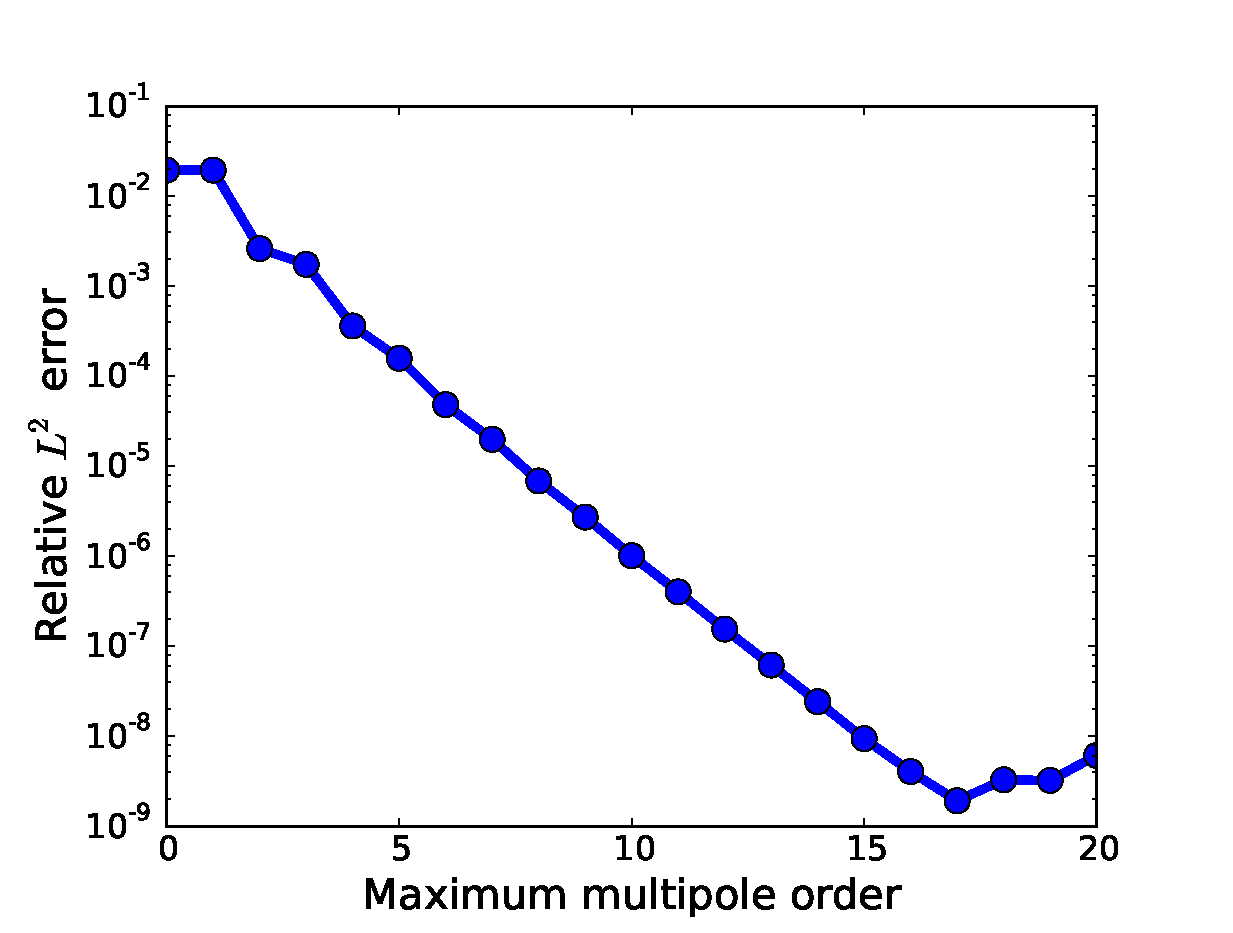
\includegraphics[scale=0.875]{plots/bc_comparison}
  \caption[Error in potential from multipole boundary conditions]
          {Error of $\Phi$ on the computational domain for a binary white dwarf simulation 
           whose boundary conditions were computed using various values of the maximum multipole order,
           relative to the exact solution determined by a brute force sum on the boundaries.
           Circles represent the error at integer values, and they have been connected by a smooth 
           line to guide the eye.\label{fig:bc_comparison}}
\end{figure}

\subsubsection{Convergence Testing}\label{sec:gravity_convergence_testing}

Since the results of a merger simulation depend strongly on gravity,
it is important to check whether proper numerical convergence is
achieved for the Poisson solver. To do so, we created a simple test
that initializes a sphere of radius $R$ and uniform mass density $\rho$
onto our grid, and used \castro\ to calculate the gravitational
potential $\Phi$ of this setup. We ensure that $R$ is an integer
multiple of the grid spacing, and the center of the sphere is at the
origin. The problem domain for our simulations is $[-1.6\ \text{cm}, 1.6\ \text{cm}]^3$, and
we take $R = 1.0\ \text{cm}$ and $\rho = 10^3\ \text{g cm}^{-3}$. 
The zones with $r > R$ are filled with an ambient material of very low density 
($10^{-8}\ \text{g cm}^{-3}$). We run this problem at multiple 
resolutions corresponding to jumps by a factor of two. For
comparison, at each grid point we evaluate the analytical potential of
a uniform sphere, which can be easily determined using Gauss' law:
\begin{equation}
  \Phi_{\text{sphere}}(r) = -\frac{GM}{r} \times \begin{cases} (3R^2 - r^2)/(2 r^2) & r \leq R \\ 1 & r > R \end{cases},\label{eq:sphere-analytical}
\end{equation}
where $M = 4\pi R^3 / 3$ is the mass of the sphere. We measure the 
numerical error by calculating the $L^2$ norm of the error and 
normalizing it by the $L^2$ norm of the analytical solution:
\begin{equation}
  \text{Error} = \frac{\|\Phi - \Phi_{\text{sphere}}\|_2}{\|\Phi_{\text{sphere}}\|_2}.
\end{equation}
We define the order of convergence $p$ between two simulations with a jump 
in resolution of integer factor $m > 1$ as
\begin{equation}
  p = \text{log}_{m}\left(\frac{\text{Error}_{\text{low}}}{\text{Error}_{\text{high}}}\right).
\end{equation}
Here $\text{Error}_{\text{low}}$ is the $L^2$ error at the lower resolution 
and $\text{Error}_{\text{high}}$ is the $L^2$ error at the higher resolution.
We expect the error to converge at $p = 2$ given the discretization we choose. 
For all simulations in this section and for all our main science simulations,
we choose a relative error tolerance of $10^{-10}$ to be satisfied in the multigrid solve.
The results of this test are plotted in \autoref{fig:gravity_convergence}. 

We find that at low resolution convergence is actually substantially better 
than second-order. The explanation for this is that we are attempting to 
model a spherical object on a rectangular grid. This results in two sources of error.
First, at very low resolution, the object does not look very spherical due to the rectangular 
grid representation, so the potential it produces is not quite that of a sphere. 
As the resolution is increased, the distribution of the mass on the grid will change.
\begin{figure}[h]
  \centering
  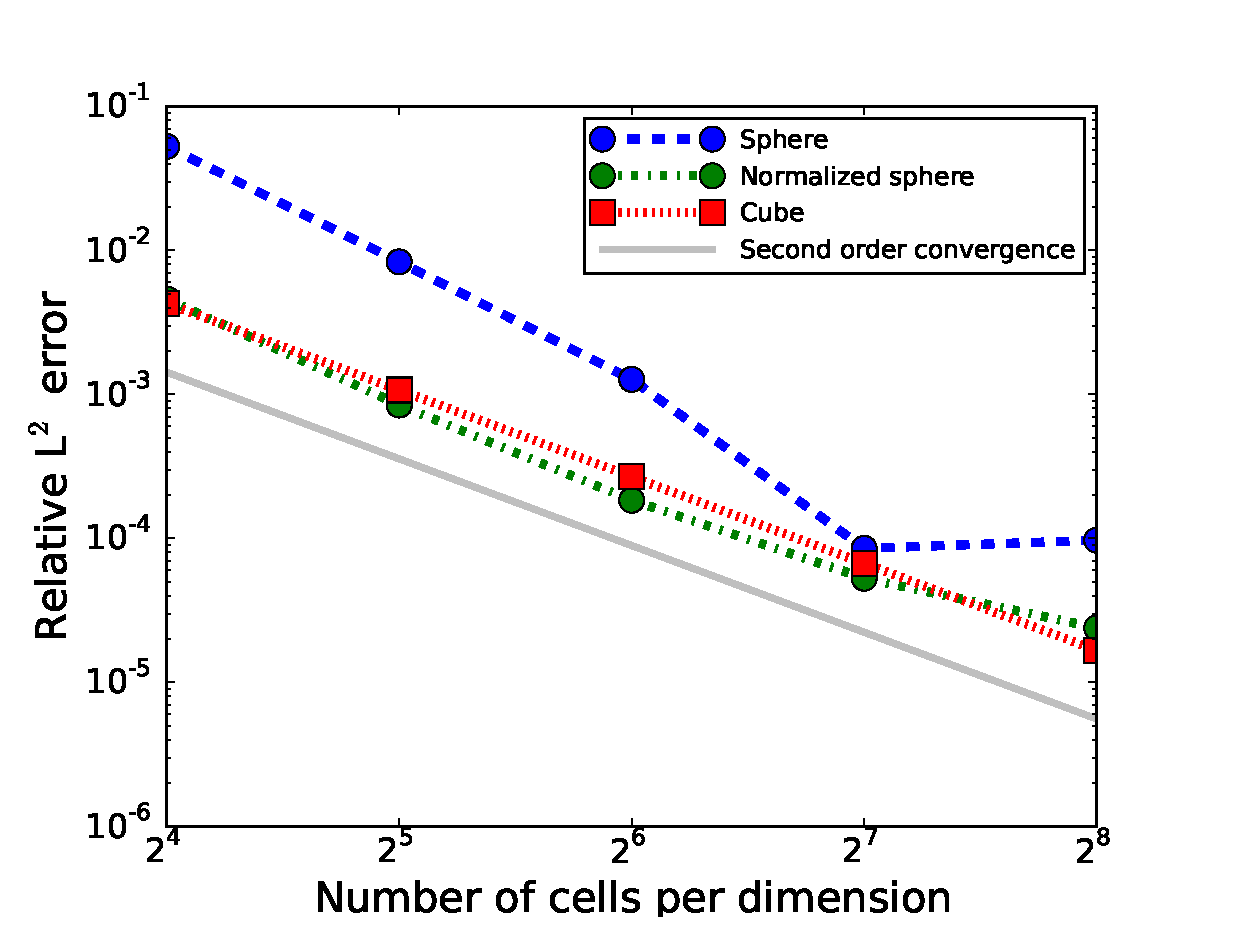
\includegraphics[scale=0.85,trim=0.075in 0.0in 0.7in 0.0in,clip]{plots/phi_comparison}
  \caption[Analytical versus numerical solution of the potential]
          {Comparison of the \castro\ gravitational potential to the analytical solution for: 
           a sphere of uniform density; the same sphere, but with the potential normalized using the 
           actual amount of mass on the grid instead of the mass of a perfect sphere; and, a 
           cube of uniform density. Plotted also is a notional curve whose slope represents
           perfect second order convergence.\label{fig:gravity_convergence}}
\end{figure}
Second, the total amount of mass on the grid will change as the sphere fills out. 
So we are combining the true accuracy bonus from increased resolution 
with the artificial accuracy bonus from getting closer to solving the problem 
we are supposed to be solving. At high resolution this effect levels off, though, 
as the representation of the sphere is not significantly different in 
our two highest resolutions shown. For example, at $128$ zones per dimension 
the amount of mass on the grid happens to be slightly closer to the true spherical 
mass than at $256$ zones per dimension.
We can eliminate the second source of error by changing the density on  
the grid so that the total mass $M$ is actually what we intend it to be.
The resolution study for this case (the ``normalized sphere'') is also
plotted in \autoref{fig:gravity_convergence}. At low resolution we still obtain
convergence slightly better than second-order, indicating that we 
have not eliminated the geometrical problem of the mass distribution changing.

The only way to fully eliminate this effect is to use a test problem that
does not change with resolution. The obvious companion problem is a cube of
uniform density $\rho$, where now $R$ is half of the side length of
the cube. At each resolution we use the same $R$ as for the sphere,
which ensures that the cube always fills exactly the same fraction of
the domain and thus has the same mass, so the only improvement comes
from better sampling at higher resolution. The gravitational potential for this
object has been worked out analytically by \citet{waldvogel:1976} (see
also a similar result by \citet{hummer:1996}, and an earlier calculation 
by \citet{macmillan:1958}). The potential is given in
Equation 15 of that paper\footnote{The last term in that equation is missing a factor of
$1/2$, which destroys the symmetry. We have inserted this missing factor and
performed a simple coordinate transformation so that the center of
the cube is at the origin.}:
\begin{align}
  \Phi_{\text{cube}}(x,y,z) &= -G\rho\sum_{i,j,k=0}^1\left[x_i y_j\, \text{tanh}^{-1}\left(\frac{z_k}{r_{ijk}}\right)\right. \notag \\
  &+ \left. y_j z_k\, \text{tanh}^{-1}\left(\frac{x_i}{r_{ijk}}\right) + z_k x_i\, \text{tanh}^{-1}\left(\frac{y_j}{r_{ijk}}\right) \right.\notag \\
  &\left. - \frac{x_i^2}{2}\,\text{tan}^{-1}\left(\frac{y_j z_k}{x_i r_{ijk}}\right) - \frac{y_j^2}{2}\,\text{tan}^{-1}\left(\frac{z_k x_i}{y_j r_{ijk}}\right) \right. \notag \\
  &- \left. \frac{z_k^2}{2}\,\text{tan}^{-1}\left(\frac{x_i y_j}{z_k r_{ijk}}\right)\right]
\end{align}
where $x_0 = R + x$, $x_1 = R - x$, $y_0 = R + y$, 
$y_1 = R - y$, $z_0 = R + z$, $z_1 = R - z$, 
and $r_{ijk} = \sqrt{x_i^2 + y_j^2 + z_k^2}$. We note that if implemented in 
\texttt{Fortran} or \texttt{C}/\texttt{C++}, the inverse hyperbolic tangent used here is
\texttt{atanh} and the inverse tangent is \texttt{atan} (\textit{not}
\texttt{atan2}). This formula is valid both inside and outside the
cube. The normalized $L^2$ error for this problem is also shown
in \autoref{fig:gravity_convergence}, and only for this problem 
do we obtain perfect second-order scaling at all resolutions.

The main lesson here is that in a convergence study, it is important
to ensure that the physical problem does not change with
resolution. Since in the case of spherical objects on rectangular
grids the effect may be to artificially boost convergence with resolution,
in a simulation with spherical objects like stars one can envision a
scenario of being fooled into believing apparently good convergence
results that are simply a convolution of artificially high
gravitational convergence and poor convergence in the hydrodynamics. A
convergence study in this case is only fully valid if there is reason
to be confident that this effect is negligible compared to other
factors.

\subsection{Rotation}
\label{sec:rotation}

For the evolution of binary systems, it is most natural to evolve the
two stars in a frame that is co-rotating at the same period as the
orbital period. Since the publication of the original code paper, \castro\ 
now has the ability to evolve systems in a rotating reference frame. 
Source terms corresponding to the Coriolis and centrifugal 
force terms are added to the momentum and energy equations. In this frame, 
the stars essentially remain stationary in their original positions due to the
centrifugal force supporting against the gravitational attraction, and
will remain this way as long as significant mass transfer does not
occur. \cite{swc:2000} demonstrated (in the context of neutron star
mergers) that conservation of angular momentum is much easier to
obtain in the rotating reference frame than in an inertial frame in
which stars advect large amounts of material around the domain. We
wish to emphasize that although it is commonly stated in the
literature that fixed-mesh codes poorly conserve angular momentum,
it is only generally true that mesh-based codes do not exactly conserve 
angular momentum when the equations are written in conservative form
for linear momentum. Indeed, \cite{motl:2002} and \cite{byerly:2014} 
have evolved binary systems using the hydrodynamics equations written 
in a form that explicitly conserves angular momentum, and it is 
straightforward to convert an existing grid-based code to solve 
the system of equations that \citeauthor{byerly:2014} present.
Additionally, the extent to which angular momentum conservation is violated in our code
is a function of the resolution. When the resolution is sufficiently high, 
excellent conservation properties can result. At reasonable resolution 
for a binary orbit our code conserves angular momentum well enough 
to keep the stars stable for a large number of orbits; however, at moderate 
resolution in an inertial frame, there is a secular loss of angular 
momentum that eventually will result in a spurious merger.
We note that as the stars begin to coalesce, the rotating reference frame
will no longer provide a good approximation to the spatial motion of
the stars and then they will begin to significantly move around the
domain. This is not necessarily problematic because the most important
feature of the rotating frame is that it helps ensure that the initial
coalescence is not the result of spurious numerical loss of angular
momentum. When significant mass transfer sets in and evolution
proceeds on a dynamical timescale, the conservation properties may be
slightly worse but angular momentum conservation is also less
important.

In a rotating reference frame with angular frequency vector $\bm{\omega}$,
the non-inertial contribution to the momentum equation is:
\begin{equation}
  \left.\frac{\partial(\rho \mathbf{u})}{\partial t}\right|_{\text{rot}} = -2\, {\bm\omega} \times (\rho\mathbf{u}) - \rho {\bm\omega} \times \left({\bm\omega} \times \mathbf{r}\right).
\end{equation}
Here $\mathbf{r}$ is the position vector with respect to the origin. Typically we choose $\bm{\omega} = (0, 0, 2\pi / T)^T$,
with the rotation axis coincident with the $z$ axis at $x = y = 0$.
$T$ is the rotation period, which is the most natural quantity to specify
for a rotating stellar system. As described in Appendix A of \cite{wdmergerI}, we include this source term
in the edge state prediction in a way that is analogous to the gravity source.
We evaluate all quantities at cell centers. We use the same predictor-corrector 
approach that we use for the gravity source terms to the momentum equations. A slight 
difference is that the Coriolis force for each velocity component is coupled to other velocity 
components. If the rotation is about the $z$-axis, then the discrete update to 
$u^{n+1}$ depends on the value of $v^{n+1}$, and vice versa. If we fix the value of 
the time-level $n+1$ quantities after coming out of the hydrodynamics update, there 
would be a slight inconsistency between the $x$ and $y$ components of the velocity. 

We propose a more accurate coupling that directly solves this implicit system of coupled 
equations. We denote by $(\widetilde{\rho \mathbf{u}})$ the value of the momentum after 
updating it with the centrifugal force, and the time-level $n$ Coriolis force. The remaining 
update for the time-level $n+1$ Coriolis force then appears as:
\begin{equation}
  (\rho \mathbf{u})^{n+1} = (\widetilde{\rho\mathbf{u}}) + \frac{\Delta t}{2} \left(-2\, {\bm\omega} \times (\rho\mathbf{u})^{n+1}\right)
\end{equation}
To proceed further, we assume that the rotation is about the $z$ axis with frequency $\omega$. 
Then there is no update to the $z$-momentum, and the other equations are:
\begin{align}
  (\rho u)^{n+1} &= (\widetilde{\rho u}) + \omega \Delta t (\rho v)^{n+1} \\
  (\rho v)^{n+1} &= (\widetilde{\rho v}) - \omega \Delta t (\rho u)^{n+1}
\end{align} 
We can directly solve this coupled system:
\begin{align}
  (\rho u)^{n+1} &= \frac{ (\widetilde{\rho u}) + \omega \Delta t (\widetilde{\rho v})}{1 + \omega^2 \Delta t^2} \\
  (\rho v)^{n+1} &= \frac{ (\widetilde{\rho v}) - \omega \Delta t (\widetilde{\rho u})}{1 + \omega^2 \Delta t^2}
\end{align}
We use this form of the momentum update in \castro. This improvement is small
but increases the accuracy of our rotating white dwarf systems over long time-scales.

The update to the energy equation can be determined by taking the dot product of the velocity
with the momentum source terms. The Coriolis term vanishes identically, and so
the Coriolis term does no work on the fluid. The update from the centrifugal force becomes
\begin{equation}
  \left.\frac{\partial(\rho E)}{\partial t}\right|_{\text{rot}} = \frac{1}{\Delta V}\int \rho \mathbf{u} \cdot \mathbf{f}^R\, dV,
\end{equation}
with $\mathbf{f}^R \equiv  -{\bm\omega} \times \left({\bm\omega} \times \mathbf{r}\right)$. 
This expression is identical in form to the gravity source under the interchange of $\mathbf{g}$ with $\mathbf{f}^R$.
As observed by \cite{marcello:2012}, we can similarly write down a rotational potential,
\begin{equation}
  \Phi^R = \frac{1}{2} \left| {\bm\omega} \times \mathbf{r} \right|^2.
\end{equation}
In the presence of rotation the conserved total energy becomes:
\begin{equation}
  \int dV (\rho E_{\text{tot}}) = \int dV \left( \rho E + \frac{1}{2} \rho \Phi + \rho \Phi^R \right).
\end{equation}
Given that we can write down a potential energy for the rotation field, then we can use the machinery of 
\autoref{sec:gravity_hydro_coupling}. We again continue to evolve explicitly an equation for 
the gas energy, and allow it to change in response to work done by or on the rotational potential.
\begin{align}
  \left.\Delta(\rho E)\right|_{\text{rot}} &= -\frac{1}{2}\sum_{f} \Delta \rho_{f} (\Phi^R_{f+1/2} - \Phi^R_{f-1/2})
\end{align}

We apply the rotational forces after the gravitational forces, but 
there is some freedom in the order in which to apply the gravitational and rotational terms.
This order may matter because the Coriolis force depends on the fluid velocity, and 
in the predictor-corrector approach, we use the velocities both at 
time-level $n$ and time-level $n+1$. If we update the latter with the gravitational force, 
then the Coriolis force sees a different velocity than the one obtained through the 
pure hydrodynamics step. (The energy equation does not face the same issue in our new formulation,
because the velocities used are always the time-level $n+1/2$ values coming from the Riemann solver.)
In practice, this does not matter significantly for our simulations in this work 
because the centrifugal force plays the dominant role in maintaining stability of non-contact 
binary systems, and the centrifugal force does not depend on the fluid velocity.
This issue may be worth exploring in future work in situations where the Coriolis 
term is non-negligible in determining the system evolution.

In all simulations performed in a rotating reference frame, we transform all relevant
quantities back to the inertial reference frame when reporting them in analysis routines 
and visualization (though the data is saved to plotfiles while still in the rotating frame). In particular,
for every zone we adjust the position, momentum, and energy to account for rotation.
If the position is $\mathbf{x}$ in the inertial frame and $\mathbf{x}^\prime$ in 
the rotating frame, and the rotation vector is $\bm{\omega}$, the transformation rules are:
\begin{align}  
  \mathbf{x}(t) &= \mathbf{R}\mathbf{x}^\prime(t) \\
  \mathbf{v}(t) &= \mathbf{v}^\prime(t) + \bm{\omega} \times \left(\mathbf{R} \mathbf{x}^\prime(t)\right)
\end{align}
The rotation matrix $\mathbf{R}$ is:
\begin{align}
  \mathbf{R} &= \mathbf{R}_z({\bm{\theta}}_3) \mathbf{R}_y({\bm{\theta}}_2) \mathbf{R}_x({\bm{\theta}}_1)
\end{align}
where $\mathbf{R}_x$, $\mathbf{R}_y$, and $\mathbf{R}_z$ are the standard rotation matrices about 
the $x$, $y$, and $z$ axes, and $\bm{\theta} = \bm{\omega} t$.



\subsection{Nuclear Network}
\label{sec:network}

White dwarfs are mainly composed of $\alpha$-chain particles, primarily ${}^4$He,
${}^{12}$C, ${}^{16}$O, ${}^{20}$Ne, and ${}^{24}$ Mg. Therefore the core of
any network appropriate for modeling nuclear burning in white dwarfs will be
these alpha chain nuclides, with the idea being that links up the $\alpha$-chain
will eventually get us to ${}^{56}$Ni, the nuclide responsible for the
energy output of Type Ia supernovae. In this paper we consider four networks
to do this, presented in order of increasing complexity. The most simple is
\isoseven\ \citep{timmes:2000}, which includes all of the aforementioned isotopes and
${}^{28}$Si (see also \citet{hix:1998}). ${}^{28}$Si effectively measures the
equilibrium state of silicon-group elements, and ${}^{56}$Ni effectively measures
the equilibrium state of iron-group elements, with the link between them governed
by the effective loss or gain of seven $\alpha$-particles. This type of network
was used by \citet{rosswog:2009} for their collision calculations in SPH.

Next is \aproxthirteen\ \citep{timmes:1999,timmes:2000}. This includes
all of the isotopes of \isoseven, and all of the $\alpha$-chain particles between
silicon and nickel (${}^{32}$S, ${}^{36}$Ar, ${}^{40}$Ca, ${}^{44}$Ti, ${}^{48}$Cr,
and ${}^{52}$Fe). This network was used by \citet{hawley:2012} and \citet{raskin:2010}.
\citet{loren-aguilar:2010} and \citet{garcia-senz:2013} used a very similar network
that included additionally ${}^{60}$Zn. The \aproxnineteen\ network \citep{timmes:1999}
builds on \aproxthirteen\ by including isotopes for hydrogen burning and explicit
tracking of photodisintegration into ${}^{54}$Fe. This network was used by
\citet{kushnir:2013}, \citet{kushnir:2014}, \citet{rosswog:2009} for their
calculations with FLASH, and \citet{papish:2015}. Finally we will also
consider \aproxtwentyone, which includes all of the above plus ${}^{56}$Cr
and ${}^{56}$Fe and related reaction links. The primary virtue of using
the latter two networks is that they allow us to track changes away from
$Y_e = 0.5$.

All four of these networks have been ported into a form that is consistent
with the \boxlib\ codes, in the freely available \microphysics\ code
repository\footnote{\microphysics\ can be obtained at \url{https://github.com/BoxLib-Codes/Microphysics}.},
a collection of microphysical routines that are designed to be used in our
hydrodynamics codes. These can be easily swapped at compile time by using the 
appropriate makefile variable.



\subsection{Nuclear Burning}
\label{sec:burning}

Given a set of nuclides and the reaction links between them, we now consider
how a burning step is performed in our software. The goal is to integrate the
vector ${\bm{Y}} = (Y_1, Y_2, \ldots, Y_n, e, T)$, where $Y_{n} = X_{n} / A_{n}$
is the molar fraction of species $n$, with $X_n$ the mass fraction and $A_n$ the
mass number of that species, $e$ is the energy released during the burn, and
$T$ is the temperature. The equation describing its evolution is given by
\begin{equation}
  \frac{d\bm{Y}}{dt} = f(\mathbf{Y}),
\end{equation}
where the components of the right-hand-side for the species come from the particular
nuclear burning network we are using. The energy release $e$ of the zone's burn
will change when the nuclear abundances evolve, according to
\begin{equation}
  \frac{\partial e}{\partial t} = N_A \sum_{n} \frac{\partial Y_{n}}{\partial t} m_{n} c^2,
\end{equation}
where $c$ is the speed of light and $m_n$ is the mass of each nuclide.

In a hydrostatic burn, we keep $\rho$ and $T$ fixed throughout, and use
the energy released at the end to compute a final temperature that is
thermodynamically consistent with the new internal energy. By contrast,
in a self-heating burn, we allow the temperature to evolve in response
to the burning (see\footnote{In the cited paper, a term based on the
thermodynamic chemical potential was included; we now believe
that it is incorrect to include such a term in the burn, since it
automatically sums to zero analytically.} \citet{maestro3}):
\begin{equation}
  \frac{dT}{dt} = \frac{1}{c_V}\frac{\partial e}{\partial t}
\end{equation}
(Although $T$ evolves during the burn so that the integration is physically
accurate, as for the hydrostatic method we discard the final value
for $T$ at the end of the burn and recompute a temperature for the zone that is
consistent with its new internal energy.) Here $c_V$ is the specific heat at
constant volume, which is provided by the equation of state.  During this burn,
we can keep $c_V$ constant using its initial value, or at each step we
can choose to re-evaluate the equation of state using the latest value of $(\rho, T)$.
The latter is more expensive but also more accurate, and we use it in this paper.
In practice we find that the cost is negligible in comparison to the more expensive
parts of the calculation, and it can significantly speed up convergence near NSE.
A third option presented by \citet{raskin:2010} is a so-called ``hybrid'' mode.
In this mode, by default we do a hydrostatic burn. If that burn fails, or if the net
energy change is negative, we do the burn again in self-heating mode. A final option
is a burn that limits the changes due to a burn to avoid numerically unstable burning.
This mode is discussed in \autoref{sec:unstable_burning} and we will call it a
``suppressed'' burn for the remainder of this work. All four options
are implemented in our burner software. The simulations shown in this work all
use the self-heating mode unless otherwise specified.

In our \microphysics\ repository we provide several software options for
solving a set of coupled stiff ODEs. For this work we use an implementation of
the well known variable-order Richardson extrapolation method presented by Stoer and
Bulirsch \cite{stoer:1980}, that is similar to the integrator which ships with
the original versions of the networks mentioned above. Previous work using the \boxlib\
codes typically used the classic \vode\ integrator \cite{vode}. We do maintain a version
of the software that is compatible with our software interfaces in the \microphysics\
repository, but we have largely shifted to integrators which are written in modern
Fortran as a consequence of our efforts to run our codes on GPUs. The Stoer and Bulirsch
integrator we provide satisfies this criterion; we also provide a rewrite of the VODE
BDF algorithm that uses modern Fortran features. The Stoer and Bulirsch algorithm
relies on a uniform relative error tolerance for all of the ODEs in the system, which
we set at $10^{-6}$ for all simulations described here.

\subsubsection{Coupling to Hydrodynamics}
\label{sec:burnerhydrocoupling}

In \castro, the reactions are coupled to the hydrodynamics using Strang splitting.
In a given timestep advance $\Delta t$, we first evolve the reactions alone through
a time interval $\Delta t / 2$. Then, we evolve the hydrodynamics for $\Delta t$,
and we evolve the reactions again for a further $\Delta t / 2$. The principal
drawback of this approach is that the reactions and the hydrodynamics can become
decoupled from each other. A common solution to this problem presented in
the literature has been to limit the size of the timestep and thereby limit the
extent of this decoupling \citep{raskin:2010,hawley:2012}, which we adopt here 
and have implemented in \castro. Defining the nuclear energy injection timescale 
$\tau_e$, and the species evolution timescale $\tau_{X_k}$,
\begin{align}
  \tau_e &\equiv \frac{e}{|\dot{e}|} \\
  \tau_{X_k} &\equiv \frac{X_k}{|\dot{X_k}|},
\end{align}
where $\dot{e}$ is an estimate of the time rate of change of the internal energy
from nuclear burning, and $\dot{X_k}$ is an estimate of the time rate of change 
of the mass fraction of the species with index $k$, we define burning-limited 
timesteps $\Delta t_{be}$ and $\Delta t_{bX_k}$:
\begin{align}
  \Delta t_{be} &= f_{e}\, \tau_e \label{eq:timestep_e}\\
  \Delta t_{bX_k} &= f_{X}\, \tau_{X_k}. \label{eq:timestep_X}
\end{align}
Given an estimate for $\dot{e}$, the factor $f_{e}$ determines by what 
fraction we would like to allow the internal energy to change
in the current timestep, under the assumption that $\dot{e}$ does not change from
timestep to timestep. Similarly, given an estimate for $\dot{X_k}$, the factor $f_{X}$ 
determines the maximum change in the mass fraction of any species. By making 
$f_{e}$ and $f_{X}$ smaller, we can control the magnitude of the decoupling 
between the reactions and the hydro. We choose by default $f_{X} = f_{e} = 0.1$, 
a choice which is slightly smaller than others in the literature. (Note that previous 
collision papers we are aware of only limited based on changes in internal energy, 
not on cahnges in species.)  The sensitivity of results to this choice will be discussed in 
\autoref{sec:collision_parameters:timestepping}. The factors $f_{e}$ and $f_{X}$ can be set at runtime in \castro.

At the start of each advance, we limit the size of the timestep to be the smaller
of the minimum hydro timestep (limited by the CFL condition), and the minimum of all the
burning timesteps across all zones. To do this, we need a method for determining 
$\dot{e}$ and $\dot{X_k}$. A typical choice in the literature has been to set, for example,
\begin{equation}
  \dot{e} = \frac{e^{n} - e^{n-1}}{\Delta t^{n-1}}, \label{eq:burning_limiter_mode_4}
\end{equation}
where is $e^n$ is the internal energy at the start of the current timestep and
$e^{n-1}$ is the internal energy at the start of the previous timestep. 
The obvious analogue is used for constructing the species rate of change.
However, there are alternative methods of constructing this derivative estimate, 
and we have found that these different methods have measurable consequences.
We define four separate methods for calculating the time derivative, with 
the above being mode 4. Mode 3 is similar to mode 4 but replaces the
denominator in \autoref{eq:burning_limiter_mode_4} with the change in 
internal energy over the last timestep only from the nuclear reactions.
Mode 2 is the same as mode 3 but we only use the change in internal 
energy from the most recent nuclear burning step, that is, the second-half
of the Strang-split burning from the last timestep (the denominator 
then becomes $\Delta t / 2$). In mode 1, the most accurate option and 
the current default in \castro, we evaluate the right-hand-side of the 
burning network given the current state to explicitly obtain the 
instantaneous value of $\dot{e}$ and $\dot{X_k}$. 

To understand the consequences of this choice, and more broadly to 
understand the limitations of Strang splitting, we consider the 
basic outline of a single-level advance in an advection-reaction system:
\begin{enumerate}
  \item Evaluate timestep $\Delta t$ for the current advance
  \item Advance the nuclear burning network by $\Delta t / 2$
  \item Advance the hydrodynamics by $\Delta t$
  \item Advance the nuclear burning network by $\Delta t / 2$
  \item Return to Step 1
\end{enumerate}
Now, consider that during a head-on collision, initial nuclear burning 
will occur at the contact point between the two stars. Because of 
the staggered updates from splitting, the evolution effectively progresses 
as a cycle between burning for $\Delta t$ and getting fresh material 
advected into the contact point by the hydro update for $\Delta t$. 
When the collision begins, $\Delta t$ is controlled by the hydrodynamic 
stability criterion, and may be large enough that it is possible for 
the burning advance in Step 4 to completely burn the freshly advected 
material all the way to NSE. Consequently the evolution is no longer 
a good approximation to smooth burning of the in-falling material but
rather separate discrete burning and hydro steps, and the nature of 
the burning evolution will be quite different. Furthermore, by the 
time we return to Step 1 and estimate the next timestep size, all 
of the burning rates will be small again, and the instantaneous 
timestep limiter of mode 1 may actually substantially overestimate 
the needed timestep. The other modes will see that the energy/species  
substantially changed over the last timestep, but will still 
overestimate the needed timestep because the burning was quiescent
for at least some portion of the last advance. In particular, our 
experience has shown that using only the energy change criterion
is particularly susceptible to this phenomenon; silicon-group 
material can build up without changing the internal energy by a 
large fraction, so the timestep limiter is never triggered, and 
then in a single step a substantial amount of iron-group elements 
can be be generated. This can have non-trivial effects on the 
total amount of iron-group elements generated over the course of
the simulation. We have found that the addition of the 
limiter based on changes in species functionally precludes this.

With the timestep limited the way we advocate in this paper, 
the timesteps are generally short enough so that the errors 
due to splitting are small. Other approaches to the coupling 
between reactions and hydrodynamics have been proposed in the 
broader literature, especially iterative methods such as 
deferred corrections that allow each of these operators to 
feel the lagged effects of the other operators. For example,
in the context of low Mach number flows, \cite{nonaka:2012} have
used the method of spectral deferred corrections \citep{SDC} to
couple their advection-diffusion-reaction equation set. In our
context this would involve using the advection as a source term
for the burning network, and symmetrically including a source
term to the hydrodynamics corresponding to the energy release
from the burning. We are presently investigating such a method,
and it may form the basis of further work on this subject.

Now we return to a point we hinted at above. The timestep
will only actually satisfy the energy criterion
$\Delta t \leq f_e \tau_e$ and species criterion
$\Delta t \leq f_{X_k} \tau_{X_k}$ when the estimates for
$\dot{e}$ and $\dot{X_k}$ we generate are at least as large
as the actual rate of change of energy and mass fractions
over the timestep. However, this can assumption can fail
during periods of runaway burning when the rate of change
of these quantities is highly nonlinear. We may not want
to neglect the errors caused by this approximation
because they may build up over an extended period of nonlinear
evolution and perhaps substantially change the final results.
To this end, we have implemented a timestep retry option in
\castro, which re-computes an advance if it violated the
stability criteria as judged from the end of the timestep.
However we have found that the benefits for this problem are
small and thus we do not use it for the simulations here.

One other point worth noting for the coupling of the reactions
and the hydrodynamics relates to the dual-energy formalism used
by \castro\ and many other hydrodynamics codes \cite{bryan:1995}.
\castro\ evolves separately equations for the total energy $(\rho E)$ and
for the internal energy $(\rho e)$. The former is conservative while the latter
is not, so for accurate hydrodynamics we prefer to use the total
energy when possible and to use the evolved internal energy variable
only in situations where the kinetic energy dominates the contribution
to the total energy. Indeed, for the cosmological purpose for which
this was originally developed, \cite{ENZO} choose a value $\eta_2 = 0.1$
so that $e$ is only updated to be equal to $E - \mathbf{v}^2/2$ if
$e > \eta_2\, E$. In other cases the evolved value of the internal
energy variable is preserved. However, this choice does not work
for our application, because the ultimate cause of the nuclear
burning in a white dwarf collision is the rapid conversion of
kinetic energy from the white dwarf bulk motion to thermal energy
as the white dwarfs slam into each other. Keeping $\eta_2$ large
prevents this from happening, and consequently the temperature
will never reach values high enough to generate significant
amounts of nickel. For this paper we choose $\eta_2 = 10^{-4}$,
which is low enough for the correct conversion of kinetic energy
but not so low that we need to be concerned about roundoff issues
caused by subtracting kinetic from total energy. This is also
the value that was used by \cite{hawley:2012}.

\subsubsection{Numerically Unstable Burning}
\label{sec:unstable_burning}

\citet{kushnir:2013} point out that an inappropriate timestep is 
not the only way for the numerical discretization to cause 
severe errors in the burning. Another failure mode is when
the energy injection timescale
$t_e$ is shorter than the sound-crossing time $t_s$ in a zone.
When the sound-crossing time is too long, energy is built up in
a zone faster than it can be advected away by pressure waves.
This is obviously a problem inherent to numerically discretized
systems as the underlying fluid equations are continuous.
This can lead to a numerically seeded detonation caused by the
temperature building up too quickly in the zone; the detonation
is spurious in this case and should be avoided if possible.
The goal is to ensure that the following condition holds:
\begin{equation}
  t_s \leq f_{s} t_e \label{eq:burning_limiter_2}
\end{equation}
The sound crossing time, $t_s$, is given by $\Delta x / c_s$, 
where $c_s$ is the sound speed and $\Delta x$ is the (minimum) 
zone width. The parameter $f_{s}$ then determines the minimum
ratio of the nuclear energy generation timescale to the 
sound-crossing time. \citet{kushnir:2013} choose $f_{s} = 0.1$ 
for their simulations, and we do too (this parameter can be set 
at runtime in \castro).

\citet{kushnir:2013} implemented this criterion by artificially 
limiting the magnitude of the energy release after a burn. We
too have developed an option for our burner to do this,
the ``suppressed'' burning mode. In a suppressed burn, we limit
the changes to the state so that \autoref{eq:burning_limiter_2}
is always satisfied. To achieve this we directly multiply the
right-hand-side vector in the integration by a constant factor $F$
for all variables, where $F$ is the multiplicative factor needed to
be applied to $\dot{e}$ such that the equality in \autoref{eq:burning_limiter_2}
holds. (If the inequality is already satisfied, then the integration
vector is not modified.) We fix $t_s$ to be the value of the sound
crossing time at the beginning of the burn (that is, we do not
update it as the sound speed changes) and we fix the energy $e$
that goes into the estimate for $t_e$ to be the value of the
internal energy of the zone at the beginning of the burn. If
instead one allowed $c_s$ and $e$ to evolve with the burn, one
would obtain a less conservative limiter in the case of explosive
burning, as $c_s$ and $e$ are both increasing in this case.
As the point of the limiter is to ensure that the changes to the
\textit{original} energy are small enough so that the following
hydrodynamics update can advect away newly generated energy
quickly enough to avoid a nuerically seeded detonation,
we desire the most conservative version of the limiter. We discuss
our results with the suppressed burning mode in \autoref{sec:collision_parameters:burningmode}.
Note that we have found that with this option enabled, it typically takes
many more timesteps to complete a burn than in self-heating mode.

Regardless of whether the suppressed burning mode works for this
particular problem, it is not physical, so in general we have
taken a different approach. If we insist that we cannot
cannot directly control the energy injection timescale, we 
must find a way to alter the sound-crossing timescale. 
We can achieve this by adding levels of refinement in 
regions that do not satisfy \autoref{eq:burning_limiter_2},
which effectively lowers the $\Delta x$ and thus the
sound-crossing time. We keep tagging zones for refinement
based on this criterion until the criterion is satisfied
on the finest level. Since the concern is regions that 
may detonate, we also tag nearby zones in a buffer region
which do not themselves satisfy the criterion,
so that a detonation in a single timestep cannot 
escape into non-refined regions. The width of the buffer 
region should thus be at least as large as the number of 
timesteps before a regridding procedure is performed.
We choose a value of two for both the number of zones in the 
buffer region and the number of steps in between regrids,
for all simulations in this paper.

While this approach may add several AMR levels 
to a simulation, we agree with \citet{kushnir:2013} that 
solving this numerical instability is crucial to avoiding
early, unphysical detonations, and so it is unavoidable
if a correct evaluation of the burning phase is desired.
A simulation that does not solve this problem in this way
(or some analogous manner) will not obtain the correct amount 
of burning, and will not converge properly with resolution. 
Fortunately, the regions where this criterion is not satisfied 
are fairly localized on the grid, so the amount of additional 
computational work is not insurmountable for a single simulation.
However, this level of accuracy may make a parameter study of
the problem challenging given current computational resources.
When resources are limited, one can still use this method and set a
limit on the number of levels of refinement possible in the simulation,
so that the refinement will still go in the right places but may not
refine all of the way to the regime of guaranteed stability. 



\newpage
\section{Simulation Software}
\label{sec:software}

\subsection{White Dwarf Models}
\label{sec:initial_models}

\subsection{Initial State}
\label{sec:initial_state}

\subsection{Analysis}
\label{sec:analysis}

\subsubsection{Gravitational Waves}
\label{sec:grvatational_waves}



\newpage
\section{Verification Tests}
\label{sec:verification}

\subsection{Maintaining Hydrostatic Equilibrium}
\label{sec:HSE}

\subsection{Gravitational Free Fall}
\label{sec:Gravitational Free Fall}

\subsection{Galilean Invariance}
\label{sec:galileo}

\subsubsection{Kelvin-Helmholtz Instability}
\label{sec:khi}

\subsubsection{Moving Star}
\label{sec:moving_star}

\subsection{Keplerian Orbit}
\label{sec:kepler}



\newpage
\section{Parallel Performance}
\label{sec:performance}



\newpage
\section{White Dwarf Collisions}
\label{sec:collisions}



\subsection{Parameter Study}
\label{sec:collisions_parameters}

\subsubsection{Timestepping}
\label{sec:collision_parameters:timestepping}

\subsubsection{Nuclear Network}
\label{sec:collision_parameters:network}

\subsubsection{Burning Mode}
\label{sec:collision_parameters:burningmode}

\subsubsection{Impact Parameter}
\label{sec:collision_parameters:impactparameter}

\subsubsection{Other Parameters}
\label{sec:collision_parameters:other}



\subsection{Resolution Dependence}
\label{sec:collisions_resolution}



\subsection{Gravitational Wave Signature}
\label{sec:collisions_gravitational_waves}



\newpage
\section{White Dwarf Mergers}
\label{sec:mergers}



\newpage
\section{Discussion and Conclusions}
\label{sec:conclusion}



\newpage
\bibliographystyle{aasjournal}
\bibliography{refs}


\newpage

\appendix



\section{Proof of Energy Conservation in Simulations using Self-Gravity}
\label{app:gravity}

In \autoref{sec:gravity_hydro_coupling}, we described our approach to updating the gas energy
in response to motions of fluid through the self-generated gravitational potential using 
\autoref{eq:grav_energy_conservation_update}. While it is straightforward to observe that this approach
should be conservative for an arbitrary fixed external potential $\Phi$, it is not as obvious that this
should be so for a self-generated potential which changes in response to mass motions on the domain. To
see that this still holds for the self-generated gravitational potential $\Phi$, let us start with 
\autoref{eq:grav_energy_conservation_update} in a slightly revised form:
\begin{equation}
  \Delta(\rho E)_i = -\frac{1}{2}\sum_{j} \Delta\rho_{ij}(\Phi_i - \Phi_{j}) \label{eq:grav_energy_conservation_update_revised}
\end{equation}
where by $\Delta \rho_{ij}$ we mean the density transferred from zone $j$ to zone $i$, so that
$\Delta \rho_{ij} = - \Delta \rho_{ji}$, and the sum is over all zone indices $j$ that are adjacent
to zone $i$. Let us define $\Phi_{ij} = \Phi_{ji} = (\Phi_{i} + \Phi_{j}) / 2$ as the potential on the
zone interface between zones $i$ and $j$. Then we have:
\begin{equation}
  \Delta(\rho E)_i = -\sum_{j} \Delta\rho_{ij}(\Phi_i - \Phi_{ij}).
\end{equation}
We can evalute the sum for all of the terms proportional to $\Phi_i$ by observing that the change in
density from time-level $n$ to time-level $n+1$ is the sum of the density fluxes from all adjacent zones.
\begin{equation*}
  \Delta(\rho E)_i = - (\rho_i^{n+1} - \rho_i^{n}) \Phi_i + \sum_{j}\Delta \rho_{ij} \ \Phi_{ij}
\end{equation*}
Now let us sum this over all zones $i$ in the domain, and ignore the domain boundaries, or assume that they are
far enough away from the region of compact support for $\rho$ that $\Phi$ is negligible there. As the second
term on the right-hand side is antisymmetric in $i$ and $j$, it cancels when summing adjacent zones, and we have:
\begin{equation*}
  \sum_{i} (\rho E)_i^{n+1} - \sum_{i} (\rho E)_i^{n} = -\frac{1}{2}\sum_{i} (\Phi_{i}^{n+1} + \Phi_{i}^{n})(\rho_i^{n+1} - \rho_i^{n})
\end{equation*}
Note that, as explained the text, we are using a time-centered $\Phi$ to correspond to the mass fluxes
at time-level $n+1/2$. Finally we re-write this in a form where the difference in total energy between time-levels
$n$ and $n+1$ is on the left-hand side and any sources causing this to be non-zero are on the right-hand side:
\begin{align}
  \sum_{i} \left(\rho E + \frac{1}{2}\rho\Phi\right)_i^{n+1} - \sum_{i} \left(\rho E + \frac{1}{2}\rho\Phi\right)_i^{n} &= \frac{1}{2}\sum_{i} \left(\Phi_i^{n+1}\rho_i^{n} - \Phi_i^{n}\rho_i^{n+1}\right) \notag \\
       &= \frac{1}{8\pi G} \sum_{i}\left(\Phi_{i}^{n+1}\nabla^2 \Phi_{i}^{n} - \Phi_i^{n}\nabla^2 \Phi_{i}^{n+1}\right) \label{eq:total_energy_difference}
\end{align}
\autoref{eq:total_energy_difference} expresses total energy conversation if and only if the right-hand side vanishes.
We observe that the right-hand side has the form of a variant of the divergence theorem often called Green's second identity:
\begin{equation}
  \int (\Phi^{n}\nabla^2 \Phi^{n+1} - \Phi^{n+1}\nabla^2 \Phi^{n}) dV = \int \left(\Phi^{n} \nabla \Phi^{n+1} - \Phi^{n+1} \nabla \Phi^{n}\right) \cdot d\mathbf{S}, \label{eq:green_second_identity}
\end{equation}
where $d\mathbf{S}$ is the area element with vector component parallel to the outward normal. The analogous result holds for the
discretized form in \autoref{eq:total_energy_difference}. With the assumptions used above, the right-hand side of
\autoref{eq:green_second_identity} will vanish as the surface integral is evaluated at infinity, where the potential
tends to zero. This concludes the proof that the method is conservative when the potential used at the zone interfaces
is time-centered, even in light of the change of the potential over the timestep due to the mass motion that is causing the change in the energy.

From the above discussion it is straightforward to see exactly why the method is not fully conservative to machine
precision in practice. First, we cannot simulate the domain out to infinity, so Green's second identity does not hold exactly
and there is some loss or addition of energy at domain boundaries. Second, \autoref{eq:total_energy_difference} holds in the
continuum limit by using the Poisson equation, but in practice it is not exactly true that $\rho_i = 4\pi G \nabla^2 \Phi_{i}$ due
to small errors in the potential at the level of the tolerances used in the Poisson solver.



\newpage
\section{Formulation of the Multipole Expansion for the Gravitational Potential}
\label{app:multipole}

The integral formulation of the gravitational potential, using a series expansion in spherical harmonics, is:
\begin{equation}
  \Phi(\mathbf{x}) = -G\sum_{l=0}^{\infty} \sum_{m=-l}^{l} \frac{4\pi}{2l+1} \int \rho(\mathbf{x}^\prime)\, Y_{lm}(\theta,\phi)\, Y_{lm}^*(\theta^\prime,\phi^\prime)\, \frac{r_{<}^{l}}{r_{>}^{l+1}}\, dV^\prime,
\end{equation}
where $\theta$ is the polar angle and $\phi$ is the azimuthal angle, $r \equiv |\mathbf{x}|$ is the radial distance, and at any point in the domain $r_{<}$ is the smaller of $r$ and $r^\prime$, and $r_{>}$ is the larger of the two. This immediately suggests writing the potential at any location as the sum of
two series:
\begin{equation*}
  \Phi(\mathbf{x}) = -G\sum_{l=0}^{\infty} \sum_{m=-l}^{l} \frac{4\pi}{2l+1}\left[ q^{L}_{lm}(\mathbf{x})\, r^{-l-1} + q^{U}_{lm}(\mathbf{x})\, r^{-l-1} \right] Y_{lm}(\theta,\phi),
\end{equation*}
where we have defined two multipole moments as integrals over the domain:
\begin{align}
  q^{L}_{lm}(\mathbf{x}) &= \int dV^\prime\, \rho(\mathbf{x}^\prime)\, Y^*(\theta^\prime,\phi^\prime)\, \Theta(r - r^\prime)\, {r^\prime}^{l} \\
  q^{U}_{lm}(\mathbf{x}) &= \int dV^\prime\, \rho(\mathbf{x}^\prime)\, Y^*(\theta^\prime,\phi^\prime)\, \Theta(r^\prime - r)\, {r^\prime}^{-l-1}.
\end{align}
$\Theta(r)$ is the standard step function, equal to one if the argument is positive and zero if the argument is negative. Geometrically,
$q^{L}(\mathbf{x})$ is an integral containing only mass interior to $|\mathbf{x}|$, and $q^{U}(\mathbf{x})$ is an integral containing only
mass exterior to $|\mathbf{x}|$. Provided that one has computed these two integrals for a point $\mathbf{x}$, one can use the series expansion
to calculate the potential at that point in principle to arbitrary accuracy by including higher order terms.
  
We prefer to work with solely real-valued quantities, and so we make use of the addition theorem for spherical harmonics \citep[Section 3.6]{jackson}:
\begin{align}
  \frac{4\pi}{2l+1} \sum_{m=-l}^{l} Y^*_{lm}(\theta^\prime,\phi^\prime)\, Y_{lm}(\theta, \phi) &= P_l(\text{cos}\, \theta) P_l(\text{cos}\, \theta^\prime) \notag \\
   &+ 2 \sum_{m=1}^{l} \frac{(l-m)!}{(l+m)!} P_{l}^{m}(\text{cos}\, \theta)\, P_{l}^{m}(\text{cos}\, \theta^\prime)\, \left[\text{cos}(m\phi)\, \text{cos}(m\phi^\prime) + \text{sin}(m\phi)\, \text{sin}(m\phi^\prime)\right].
 \end{align}
The $P_l(x)$ are the Legendre polynomials and the $P_l^m(x)$ are the associated Legendre polynomials. We construct them using a stable recurrence relation given known values for $l = 0$ and $l = 1$. We can then formulate the expansion in a different way:
\begin{align}
  \Phi(\mathbf{x}) &= -G\sum_{l=0}^{\infty} \left\{ Q_{l}^{(L,0)}(\mathbf{x})\, P_l(\text{cos}\, \theta)\, r^{-l-1} + Q_{l}^{(U,0)}(\mathbf{x})\, P_l(\text{cos}\, \theta)\, r^{l} \right. \notag \\
  &\hspace{0.7in} + \sum_{m=1}^{l} \left[ Q_{lm}^{(L,C)}(\mathbf{x})\, \text{cos}(m\phi) + Q_{lm}^{(L,S)}(\mathbf{x})\, \text{sin}(m\phi)\right] P_{l}^{m}(\text{cos}\, \theta)\, r^{-l-1} \notag \\
  &\hspace{0.7in} + \left. \sum_{m=1}^{l} \left[ Q_{lm}^{(U,C)}(\mathbf{x})\, \text{cos}(m\phi) + Q_{lm}^{(U,S)}(\mathbf{x})\, \text{sin}(m\phi)\right] P_{l}^{m}(\text{cos}\, \theta)\, r^{l} \right\}
\end{align}

The multipole moments now take the form:
\begin{align}
  Q_l^{(L,0)}(\mathbf{x}) &= \int P_l(\text{cos}\, \theta^\prime)\, \Theta(r - r^\prime)\, {r^{\prime}}^l \rho(\mathbf{x}^\prime)\, d^3 x^\prime \\
  Q_l^{(U,0)}(\mathbf{x}) &= \int P_l(\text{cos}\, \theta^\prime)\, \Theta(r^\prime - r)\, {r^{\prime}}^l \rho(\mathbf{x}^\prime)\, d^3 x^\prime \\  
  Q_{lm}^{(L,C)} &= 2\frac{(l-m)!}{(l+m)!} \int P_{l}^{m}(\text{cos}\, \theta^\prime)\, \text{cos}(m\phi^\prime)\, \Theta(r - r^\prime)\, {r^\prime}^l \rho(\mathbf{x}^\prime)\, d^3 x^\prime \\
  Q_{lm}^{(U,C)} &= 2\frac{(l-m)!}{(l+m)!} \int P_{l}^{m}(\text{cos}\, \theta^\prime)\, \text{cos}(m\phi^\prime)\, \Theta(r^\prime - r)\, {r^\prime}^{-l-1} \rho(\mathbf{x}^\prime)\, d^3 x^\prime \\
  Q_{lm}^{(L,S)} &= 2\frac{(l-m)!}{(l+m)!} \int P_{l}^{m}(\text{cos}\, \theta^\prime)\, \text{sin}(m\phi^\prime)\, \Theta(r - r^\prime)\, {r^\prime}^l \rho(\mathbf{x}^\prime)\, d^3 x^\prime \\
  Q_{lm}^{(U,S)} &= 2\frac{(l-m)!}{(l+m)!} \int P_{l}^{m}(\text{cos}\, \theta^\prime)\, \text{sin}(m\phi^\prime)\, \Theta(r^\prime - r)\, {r^\prime}^{-l-1} \rho(\mathbf{x}^\prime)\, d^3 x^\prime.  
\end{align}
In practice, of course, we select some maximum value $l_{\text{max}}$ at which we terminate the summation, determined either by computational efficiency requirements or by the fact that there is little information at high orders for sufficiently smooth mass distributions. In \castro\ we have the capability to compute any of the above multipole moments, though in this paper we are only using the multipole expansion to calculate the boundary conditions on the potential, and so we neglect calculation of the moments with a $U$ subscript as we are assuming that all of the mass is interior to the boundary. \autoref{eq:multipole_potential} is directly recovered under these conditions.

\clearpage

\end{document}
